\chapter*{Листа на кратенки}
\addcontentsline{toc}{chapter}{Листа на кратенки}  

\begin{itemize}
    \item MIT - Massachusetts Institute of Technology - анг. Институт за технологија на Масачусетс
    \item MIDI - Musical Instrument Digital Interface - анг. Дигитален интерфејс за музички инструменти
    \item CNN - Convolutional Neural Network - анг. Конволуцискa Невронскa Мрежa
    \item RNN - Recurrent Neural Network - анг. Рекурентнa Невронскa Мрежa
    \item RBM - Restricted Boltzmann Machines - анг. Ограничени Болзманови Машини
    \item LSTM - Long Short-Term Memory - анг. Долга Краткорочна Меморија
    \item BPTT - Back-Propagation Through Time - анг. Пренос на грешка назад низ времето
    \item TBPTT - Truncated Back-Propagation Through Time - анг. Скратен пренос на грешка назад низ времето
    \item VRASH - Variational Recurrent Autoencoder Supported By History - анг. Варијациски автоенкодер поддржан од историја
    \item GAN - Generative Adversarial Networks - анг. Генеративни Непријателски Мрежи
    \item NADE - Neural Autoregressive Distribution Estimator - анг. Невронски авторегресивен естиматор на веројатностна дистрибуција
    \item RTRBM - Recurrent Temporal RBM - анг. Рекурентна временска ограничена болцманова машина
    \item DBN - Deep Belief Network - анг. Длабока мрежа на доверба
    \item ReLU - Rectified Linear Unit - анг. Исправена линеарна единица 
    \item Adam - Adaptive Momentum Estimator - анг. Адаптибилен естиматор на импулс
\end{itemize}

\newpage

\chapter{Вовед}

Генерирање на музика и други типови на мултимедиска содржина се мошне популарни теми на истражување во денешно време. Во академијата и популарните дискусии се води дебата за возможноста за оспособување на компјутерски систем да покаже знаци на креативност, како што може да се види во трудот \cite{Ghedini2015}. Едната страна на дебатата тврди дека компјутерите нема да можат, барем не во скоро време, да креираат ништо уникатно и имагинативно бидејќи сите компјутерски системи за креирање на музика би зависеле од некој модел изграден со користење колекција од композици направени од човек, или пак правила или граматики креирани од човек. Ваквите системи би работеле со некаков произволно апстрактен и комплексен систем на комбинации и рекомбинации за креирање на нови дела. Ова може да се смета како клучен лимитирачки фактор за израз на имагинација и инвентивност. Другата страна на дебатата не смета дека ова е ограничување, туку како неопходно зло или како еволутивен чекор во развивање на компјутерска креативност, исто како што тоа е дел и од развојот на секој човек. Најголемиот дел од луѓето стапуваат во контакт со музиката долго време пред да започнат самите да допринесуваат кон целокупното човечко творештво. Така, во делата на секој творец може да се пронајдат свесни и несвесни влијанија од други автори со чии дела ги имаат запознаено. Имитацијата е основен елеменет во процесот на учење, како и форма на оддавање почит. Врз основа на ова, пропонентите на компјутерската креативност тврдат дека ваквите ограничувања се во најлош случај само еволутивен чекор.

Во последните десеттина години настана револуција во полето на машинската интелигенција. Драстичното зголемување на компјутерската пресметковна моќ со искористување на компјутерските графички адаптери и модели за масовно паралелно процесирање го овозможи практичното искористување на голем број на алгоритми и техники кои претходно даваа релативно слаби резултати поради невозможноста за обработување на голем број податоци во ограничен временски рок. Длабоко учење е една подгрупа од таквите алгоритми и техники која во последно време се покажува како најпопуларна и ефективна. Таа се темели на искористување на тн. длабоки невронски мрежи, кои се конструирани како аналогија на човечкиот ум. Градбени едники им се тн. неврони кои го имитираат функционирањето на биолошките неврони, организирани во слоеви. Длабоки се невронските мрежи кои се изградени од повеќе слоеви од неврони. Различни организации на длабоки невронски мрежи се покажаа многу ефективни за работа со различни податочни типови, како на пр: слики, видео, историски податоци (временски серии), текст итн. Главната цел на трудов е да се искористат алгоритми за машинско учење, поточно длабоко учење, кон решавање на проблемот на компјутерско генерирање на музика.

Уште пред започнување со изработка, беше јасно дека било каков генеративен систем со модели за машинско учење има огромен потенцијал за тесно грло бидејќи не постои начин за квалитативно оценување на излезот од таков модел, т.е. не постои целна функција која што може да се оптимизира во процесот на учење. Во наведените трудови во поглавје \ref{ch:pregled}, најчест пристап е рачна евалуација на резултатите од страна на човек, којшто во принцип треба да е музички образован. Ваквото тесно грло не само што елиминира гаранција за квалитет на резултатите, туку и го ограничува изборот на алгоритми за машинско учење. 

Досегашните обиди за генерирање на музика може да се поделат на две категории: генерирање на пишана музика и генерирање на аудио сигнал. Пристапите за пишана музика значително варираат во комплексноста на проблемот што пробуваат да го решат, тргнувајќи од генеирање на „12 bar blues“ \cite{Eck2002} блуз во 12 такти, до народна музика \cite{Sturm2016}, па се до Бахови корали во 4 гласа \cite{Liang2017,Hadjeres2016}. Во другата категорија, досегашните обиди \cite{Oord2016} се ограничени до учење на звучен сигнал од еден инструмент со ограничена должина, или работат со голема улога на човечки композитор \cite{Ghedini2015}. Поконкретно целта на овој труд беше генерирање на пишана полифона музика со модели за машинско учење. Не беа поставени додатни структурни ограничувања од самиот почеток, освен музиката да е од ист или сличен жанр и од еден автор или мал број на автори.

Во трудот е прикажана нашата работа на полето на генеративни музички модели, и преглед на постигнати резултати и плановите за иднина. Трудот е организиран во следните поглавја: во поглавјето \ref{ch:motivacija} е изложена нашата мотивацијата за превземање на истражувањето и е дефинирана целта што треба да се постигне, во поглавјето \ref{ch:pregled} е даден преглед на досегашните решенија, во поглавјето \ref{ch:pristap} се систематизирани досегашните пристапи за генерирање на пишана музика, во поглавјето \ref{ch:masinsko} е даден преглед на алатки и техники од машинско учење релевантни за трудот, во поглавјето \ref{ch:evaluacija} се изложени проблемите со објективна евалуација на генеративните резултати, во поглавјето \ref{ch:podatoci} е даден преглед на музичките податочни формати и нивната репрезентација за модели за машинско учење, во поглавјето \ref{ch:alatki} се опишани искористените алатки, поглавјето \ref{ch:studija} е студија на случај во која е опишан нашиот обид за генерирање на музика со модел за машинско учење, и во последното \ref{ch:zaklucok} поглавје е заклучен трудот и се изложени можностите за подобрување кои беа увидени.

\chapter{Мотивација и дефиниција на проблемот}
\label{ch:motivacija}

Андреј Карпати со статија „Неразумната ефективност на рекурентните невронски мрежи“ \cite{AndrejKarpathy2015} значително го зголеми интересот на полето на машинско учење, поточно длабоко учење со невронските мрежи и нивните рекурентните варијанти. Во статијата е прикажан генеративен јазичен модел на ниво на буква, составен од длабока невронска мрежа изградена од рекурентни ќелии (рекурентна невронска мрежа), истрениран на повеќе колекции на текстови од различен карактер (есеи од Пол Греам, драми од Шекспир, XML од статии од Википедија, LaTeX текстови и C++ изворен код). Моделот ги учи текстовите буква по буква, и резултатот го генерира на истиот начин. Иако не му се додаваат никакви информации за структурата на текстовите, на јазикот, граматички правила или форматирање, тој успева да генерира резултати кои се конформираат во голема мера кон изворниот формат. Самиот креира ад-хок правила за конструкција на сложени зборови, генерирајки и сложени зборови што ги нема во изворните текстови, учи употреба на сврзници, честички, негации, сложени реченици иако не секогаш се поврзани составните прости реченици и сл. Во случајот каде што учи технички документи и изворен код ги следи и долгорочните зависности на отворање и соодветно затворења на загради и XML маркери кои често се простираат на растојание од повеќе стотини елементи низ текстот. Успешноста на овој модел има инспирирано огромен број на истражувачи и луѓе од индустријата да се обидат да креираат генеративни модели со користење на рекурентни невронски мрежи со релативно едноставни архитектури. 

Оваа статијата служеше за инспирација за употреба на техники за длабоко учење и техники за обработка на природни јазици за креирање на модел за генерирање на полифона музика. Моделот треба да биде јазичен модел на ниво на буква, и музиката да ја третира апстрактно како текст, со можност за додатни информации врз основа на музичка теорија. Користење на јазичен модел треба да овозможи и користење на техники за обработка на природни јазици. Од архитектурите за длабоко учење идејата беше да се искористат рекурентни невронски мрежи поради нивната способност за учење на произволно долги секвенци. Музиката треба да биде полифона, т.е. да има повеќегласност составено од ритам и мелодија, и доколку е возможно составните елементи да поддржуваат акорди и поединечни ноти.

Покрај можноста за придонес кон филозофската дискусија за компјутерската креативност, увидени беа и повеќе можности за практично искористување на систем за генерирање на музика, вклучувајки:
\begin{itemize}
\item Музика за видео игри, т.е. процедурално генерирана музика, кадешто музката ќе се адаптира на атмосферата и претходно дефинирани параметри, темпо и сл.
\item Музика за вежбање. Во принцип генерирање на музика што треба да следи предефинирани рутини за вежбање и ќе помага во одржување на темпо и енергетско ниво и ќе го стимулира корисникот. Додатно ритамот и темпото на музиката може да бидат и под влијание на виталните знаци на корисникот, примарно пулс и дишење.
\item Компјутерски помогнато компонирање на музика. Човечки композитор би ја користел апликација која му овозможува дополнување на музика, варијација на постоечка музика според параметри итн.
\end{itemize}

\chapter{Преглед на литературата}
\label{ch:pregled}

Еден од најраните обиди за „алгоритамско“ креирање на музика познат како „Музички игри со коцки“, бил популарен во XVIII век. Првата забележана композиција создадена на овој начин е „Секогаш подготвен менует и полонески композитор“ (гер. Der allezeit fertige Menuetten- und Polonaisencomponist) од Јохан Филип Кирнбергер во 1757 год. Најпопуларни биле игрите напишани од страна на Хајдн и Моцарт, поради што може да се пронајдат вакви игри и под името Моцартови коцки. Ваквите игри најчесто се состојат од табели од музички исечоци, во големина од еден до неколку такта, кои се напишани така што ќе немаат остри рабови за да може лесно да се надоврзуваат. Играчите фрлаат коцки или случајно избираат број, па според тоа избираат исечок од табелата според одредена шема која оди заедно со табелата, а избраниот исечок потоа го прилепуваат на композицијата. Играта трае се додека играчот не одлучи дека има доволно долга композиција. Квалитетот на добиената композиција зависи најмногу од квалитетот на исечоците. Бројот на можни исечоци мора да биде релативно мал за да може играчите практично да играат, а да не прелистуваат стотици страници секој пат кога ќе ги свртат коцките. За да можат да бидат исечоците лесно поврзливи од двете страни треба да имаа почеток, средина и крај, т.е. да бидат самостојни микро-композиции. Поради сите овие ограничувања, музичките игри со коцки повеќе се едноставна игра отколку практичен начин за алгоритамски пристап за компонирање музика. Доколку се решат ограничувањата на играта, таа би добила многу поголем капацитет за изразување на креативност. Таквата игра би била непрактична за човечка употреба, но не и за компутерски имплементации. Скоро сите истражени пристапи може да се апстрахираат како играта врз основа на 2 клучни точки:
\begin{itemize}
    \item Дефиниција на исечок / Основен елемент на композиција 
    \item Избор на исечок / Начин на прилепување на исечоците
\end{itemize}
Тие може да се поделат во две епохи, и тоа: пред длабоко учење и со длабоко учење. Пред длабоко учење сите пристапи се блиски до игрите со коцки, само го заменуваат процесот на избор на исечок со: правила и граматики, експертски системи, генетски алгоритми. Пристапите со длабоко учење не со толку слични со музичките игрите, но суштински го вршат истото. 

\section{Граматички / експертски системи} 

Д. Коуп во трудот \cite{Cope1991} ја опишува првата компјутерска имплементација на музичките игри со коцки. Коцките се заменети со стохастички процес. Исечоците се претставени со шаблони, кои ги добиваат со делење на корпус од пишана музика во должини од еден до два такта. Шаблоните се анализираат според рачно пишани правила базирани на музичка теорија, и содржат „потпис“ на авторот и се чуваат во лексикон. Случајниот процес бираат од кандидат шаблоните од лексиконот, коишто се компатибилни со претходно избраниот шаблон. Компатибилоста ја одредуваат со анализа на тон и должина на ноти и со споредба на шаблони, којашто се врши врз основа на релативно движење на тоновите и должините.

Имплемнтација на играта со генетски алгоритам може да се види во трудот \cite{Biles1994}. Тука исечоците се претставени со хромозоми. Музиката е во строг 4/4 ритам, а секој хромозом е еден такт составен од 8 настани во должина од 1/8, при што настан може да бидат нова нота, задржување на стара нота и пауза. Квалитетот на секој од хромозомите при процесот на еволуција се одредува рачно од страна на човечки ментор, кој внесува вредност со помош на тастатура. Ова е очигледна болна точка за практичноста на алгоритамот, што го прави крајно непрактичен. Потребно е многу време за вешт ментор да ги преслуша и оцени кандидатите. 

Во трудот \cite{Zils2001} авторите опишуваат експертски систем за креирање на мозаик од музички сегменти (исечоци). Сегментите се опишани со множество на дескриптори. Дефинираат два вида на правила: сегментни, т.е. правила кои што се евалуираат на ниво на сегмент, и секвенцни, т.е. глобални правила, коишто се евалуираат на целата секвенца. Дел од правилата се претходно дефинирани, а дел корисникот на алгоритмот ги внесува рачно. Доколку сака, корисникот може и да избере готова песна врз основа на која ќе се екстрахираат правила со кои ќе биде креирана нова песна, во суштина имитирајќи ја оригиналната песна од високо ниво. Бидејќи правилата не секогаш се во согласување, авторите имаат и дефинирано постапка за евалуација на важноста на правилата врз основа на тежини, т.е. функција на чинење која ја минимизираат при процесот на генерирање.

Пристапот опишан во трудот \cite{GarciaSalas2011} може наједноставно да се објасни како n-gram модел или модел со Маркови синџири. Системот се состои од дел за учење и дел за компонирање. Делот за учење генерира правила врз основа на податочното множество, а делот за компонирање генерира нова музика врз основа на правилата и има повратна врска кон делот за учење. Правилата се изразени преку 3 матрици: матрица на времетраења на нотите, локална матрица на фрекфенции и кумулативна матрица на фрекфенции. Овие матрици се пополнуваат според n-gram фрекфенции на појавување во податочното множество. Алгоритамот за генерирање пресметува матрица на веројатност на појавување како функција од претходно споменатите матрици. Генерирањето се врши со стохастичен процес врз основа на матрицата на веројатности. 

Уште еден систем за градење на музички мозаици може да се види во трудот \cite{Schwarz2006}, кадешто авторите имаат изградено корпус од кратки исечоци, секој опишан со одредено множество на дескриптори, наголем дел добиени со математички трансформации на аудио сигналот (пр. брзи фуриеви трансформации, гаворови бранови, хистограми и сл.). Системот има алгоритам за избирање на исечоци, кои последователно ги прилепува за време на процесот на генерирање. Алгоритамот е базиран на човечки зададени правила или имитација на постоечки песни, кадешто алгоритамот само ги бира исечоците кои ги задоволуваат критериумите базирани на десктрипторите, без да води сметка за колку добро се сложуваат меѓусебе, и врши благо измазнување на краевите помеѓу исечоците.

\section{Алгоритми со длабоко учење} 

Голем број на алгоритми и техники измислени дури од самите почетоци на истражување на полето на машинско учење, како што се модели со невронски мрежи, машини со носечки вектори, дрва на одлука и сл., во минатото не покажувал резултати конкурентни на рачно изградени експертски модели. Најголемо ограничување беа пресметковната моќ и меморискиот капацитет на машините на коишто се извршуваа моделите, што ја ограничуваше големината и комплексноста на моделите како и количината на податоци што може да се обработи при учење на истите. Меѓутоа, во последните десетина години започнаа да се користат графичките акцелератори (попознати како графички картички) за општа намена (GPGPU - General Purpouse GPU). На сцена се појавија две библиотеки CUDA и OpenCL кои овозможуваат користење на графичките акцелератори за секакви пресметковни намени, што се покажа многу корисно за развивање на модели за машинско учење. Оттогаш се појави и експлозивен интерес за изстражување на секакви теми и решавање на секакви проблеми со користење машинско учење, вклучувајќи и модели за компјутерско генерирање на музика. Самото зголемување на пресметковна моќ овозможува создавање на многу подлабок, пософистициран и поапстрактен систем од тоа што го нудеа претходно споменатите техники. Во продолжение следува преглед на повеќе пристапи за генерирање на музика со длабоко учење, кое претставува подмножество на техники за машинско учење со користење на длабоки невронски мрежи.

Првиот документиран обид за користење на невронски мрежи за генерирање на музика е од страна на Д. Ек во трудот \cite{Eck2002}. Целта им била тренирање на модел кој ќе генерира блуз во 12 такта. Музиката се состои од 2 оделни компоненти, секвенца на акорди која го одредуваат ритамот и ја даваат основната структура на музиката и мелодиска линија. Моделот има две групи од по 4 пара LSTM ќелии (рекурентни неврони), од кои едната е задолжена за учење на мелодијата, а другата за акордната секвенца. Музиката ја преставуваат во тн. репрезентација во пијано лента. Музиката има строга дефинирана структура, 12 такта, 4/4 ритам, а времето е подделено на 1/8 ноти. Моделот го искористиле во два експерименти, во првиот тој ја учи само секвенцата на акорди, а во вториот и акордите и мелодијата. Тренирањето е извршено со крос-ентропија фунција за загуба, со сигмоидална функција на активација. Делот за учење на акорди ја споделува својата внатрешна состојба со делот за учење на мелодија. Авторот смета дека системот генерира добра музика, но сепак проблемот што пробува да го реши е хипер фокусиран и ограничен. Трудот \cite{Eck2008} претставува надоградување на претходно опишаниот систем. Го нема веќе фокусот на блуз во 12 такти, туку работат со податочно множество од поразлични MIDI датотеки, зголемена е комплексноста на моделот, со многу повеќе ќелии и повеќе слоеви од истите. Додатно на моделот му прикажуваат и временски задоцнети копии од податоците, на семантички важни растојанија. Задоцнетите временски копии ги додале под хипотезата дека во музиката значајни настани се случуваат на метрички важни места како што се почетокот и крајот на тактовите, како и на моменти зависни од ритамот (пример во македонскиот 7/8 ритам ен-два-три, ен-два, ен-два, има значајни транзиции на секое „ен“). Ова го постигнуваат со проширување на пијано лентата такашто при секој чекор на моделот му се прикаже лентата од тековниот временски чекор, и од чекорите на претходно зададени интервали, како на пр. пред 1, 4 и 16 такта точно на истиот удар во тактовите. Покрај LSTM слоеви моделот има и паралелен целосно поврзан слој неврони којшто треба да помогне во учење на локални зависности меѓу нотите. Мрежата ги учи песните како една секвенца, со што акумулираната грешка при учење се ресетира на границата помеѓу песните. Нотите се ограничени помеѓу C3 и C5 и сите песни се транспонирани во ист клуч. Податочното множество е изградено од  ирски народни песни во 4/4 ритам. Моделот генерира нови песни со предвидување на следната нота откако ќе се припреми со исечок од постоечка песна.

Во трудот \cite{Sturm2016} авторите користат техники од обработка на природни јазици за генерирање на музика. Карактеристична е употребата на форматот за музика познат како ABC. Форматот е текстуален, наменет примарно за запишување на изворна музика на едноставен и лесно разбирлив начин за луѓето, содржи мелодиска линија запишана со основни тонови и пропратен тескт. Музиката пишана во овој формат е опишана на високо ниво и доста стилски хомогена. Сите овие фактори ги прават форматот и податочното множество одлични за обработка со техники за обработка на природни јазици. Со користење на многу едноставен јазичен модел на ниво на буква и едноставна архитектура од 3 слоја од 512 LSTM неврони, со софтмакс активациски слој авторите добиле многу позитивни резултати. Во трудот прикажуваат и додатно подобрување на системот со повеќе чекори на предпроцесирање на текстот, со користење на ограничено семантичко музичко знаење, со кои го трансформираат текстот од низа букви во низа уникатни и музички значајни токени врз основа на музичката функција на буквите/симболите. Додатно извршиле и процес на селекција и стандардизација на множеството песни за да ги исфрлат песните коишто се: премногу кратки, недволно информативни, конфузни или двосмислени; и транскрипција на сите песни во ист клуч. Моделот е трениран со множество од над 23000 песни, во мини-бечови од 50 елементи, во 100 епохи. Генерирањето се врши со итеративна постапка, започнувајќи со посебен симбол за старт. Имаат извршено додатен експеримент во кој го стартуваат моделот со подолг извадок од песни од одредени автори за да ги проверат можностите на моделот да генерализира стилски карактеристки, и авторите тврдат дека моделот е способен за тоа.

Врз основа на техники за обработка на природни јазици може да се направат и модели на ниво на збор. Ваков пристап си има свои ограничувања бидејќи се зголемува драстично бројот на основни елементи, има многу повеќе зборови одколку букви и симболи во јазициите, и нивните фрекфенции на појавување опаѓаат драстично. За да се надмине ова се користат различни техники за намалување на бројот на променливи во системот, т.е. намалување на бројот на зборови, групирање на зборовите според функција, споделување на веројатности помеѓу зборовите и трансформации во помалку димензионален простор. Токму ваков пристап може да се види во \cite{Bretan2016}, каде што авторите работат со исечоци од 1 до 4 такта. Бидејќи има огромен број на можни варијации на таквите исечоци истите ги смалуваат во помалку димензионален простор користејќи ја техниката на вградување во латентен простор (анг. latent space embedding). Вградувањето го вршат врз основа на множество од дескриптори со кои ги опишуваат исечоците. Со ова се добива структура налик на хеш табела, само со повеќе можни резултати при процесот на декодирање на елемент во табела во исечок. Тренирале два модела, еден што учи секвенци од репрезентации на зборовите, а друг што ги учи песните на ниво на буква и е наменет за олеснување на декодирањето, т.е. ги гледа работиве помеѓу тековната секвенца и сите потенцијални декодирани исечоци, и одредува компатиблиност на последователни исечоци. Намената на моделот на ниво на збор е да учи музички зависности на подолг временски период, во обид да се научи структура на цела песна, додека другиот модел ги учи локалните зависности помеѓу нотите. На крај извршиле субјективна евалуација од страна на 32 музички експерти, коишто ги рангирале резултатите од повеќе инстанци на моделот со различн параметри.

Коралите на Јохан Себастијан Бах претставуваат интересен проблем за моделирање. Се стостојат од 4 гласна полифонија, алто, тенор, сопрано и бас монофони мелодиски линии. Може да се моделираат на сличен начин како акордите, со тоа што зависностите помеѓу гласовите не е иста како меѓу нотите во акордите. Исто така уникатните комбинации од ноти по гласови поретко се јавуваат одошто кај акордите, бидејќи акордите се стандардни конструктивни елементи во музиката. Ова податочно множество е главен фокус на трудовите \cite{Liang2017, Hadjeres2016}. Во трудот \cite{Liang2017} е искористена релативно еднсотавна архитектура, составена од повеќе рекурентни LSTM слоеви, со слоја вградување по влезниот инспириран од word2vec \cite{Herremans2017}, со едноставен софтмакс активациски слој. Бидејќи ритамот во целото податочно множество е 4/4, музиката е поделена на еднакво долги рамки со времетраење $1/16$ нота, во која 4-те гласа се претставени со секвенца од поединечни ноти, а рамките меѓусебно се поделени со посебен симбол за разграничување. Така ја намалиле комплексноста на проблемот за предвидување од $O(128^4)$ на $O(128)$, но ја издолжуваат секвенцата со фактор 5. Со алгоритам за оптимизација на хиперпараметри GridSearch ги оптимизирале следните парамерти: број на рекурентни слоеви, големина на рекурентните слоеви, големина на слојот за врадување, должина на секвенца што се користи за TBPT, процент за dropout техника за нормализација. Во трудот \cite{Hadjeres2016} авторите користат посебни модели за секој од гласовите, и на крај ги сумираат нивните резултати. На тој начин се претпоставува одредена независност помеѓу гласовите, иако тие се функционално зависни помеѓусебе. Паралелно ги обработуваат тековниот временски чекор, повеќе временски чекори наназад и нанапред, во хетероген модел составен од рекурентни и не-рекурентни невронски слоеви. Податочното множество го имаат транспонирано во сите можни клучеви наместо стандардизирање кон еден клуч. И во двата труда се прикажани процеси за субјективна евалуација на резултатите со онлајн тестови каде што на корисниците им се пушта музички исечок и треба да одлучат дали музиката е генерирана или оригинална композиција на Бах. Во двата случаја најпозитивни резултати покажале кога моделите ги користеле за рехармонизација на мелодија врз основа на 2 или 3 постоечки гласа.

Во системот наречен „Производ на експерти“ предложен во трудот \cite{Johnson2017} се користат два прости јазични модели во тандем, тренирани на истото податочно множество од џез песни, со различен перспектива врз истото. Двата модела се едноставни рекурентни длабоки невронски мрежи, од кои едниот ги гледа песните како секвенца од релативно движење на мелодијата, т.е. при секој чекор ја гледа апсолутната разлика во тонот меѓу последователни ноти, додека другиот ја следи хармониската улога на нотата во тековниот акорд од прогесијата на акорди. Двата модели при секој чекор моделираат веројатностна дистрибуција и се тренираат со оптимизациски алгоритми за намалување на крос-ентропија. Финалниот резултат е параметризирана сума од двете веројатностни дистрибуции. Тренирањето и генерирањето на песните следи стандардна итеративна процедура.

Користењето на јазични модели на ниво на буква овозможува едноставно моделирање на монофона музика. При моделирање на акорди со пијано лента се појавува проблем на енумерирање сите можни конфигурации на ноти што може да се појават, пр. за гитара има грубо $2*24^6$ можни конфигурации на ноти. Еден пристап за намалување на проблемите што доаѓаат од зголемена димензионалност може да се види во \cite{Boulanger-Lewandowski2012, Boulanger-Lewandowski2014, Goel2014}, каде што авторите користат хибридни архитектури, изградени од рекурентни невронски слоеви во различни комбинации со енергетски модели. Идејата е да се искористат особеностите на енергетските модели, како што се RBM и NADE, да моделираат веројатностни дистрибуции, кон моделирање на истовремено појавување на нотите во акорди. Од трудовите \cite{Boulanger-Lewandowski2012, Boulanger-Lewandowski2014} произлегуваат моделите: RTRBM, RNN-RBM, RNN-NADE, од кои RNN-NADE се покажал како наједноставен за тренирање и со најдобри генеративни резултати, а истовремено и најекспресивен, и покрај тоа што од енергетските модели NADE има релативно помала експресивна моќ. Моделот може да се разбере како низа од условени енергетски слоеви, по еден за секој временските чекори што го обработува мрежата, со излез во детерминистички рекурентен невронски слој. Наголем проблем на овој тип на модели се покажала осетливоста на иницијална состојба, што многу ја потенцира важноста на пред-тренирање при нивна употреба. Моделот се покажал успешен во моделирање на локални зависности, хармониски правила и кратки мелодиски линии, меѓутоа не може да моделира долговременски зависности. Во трудот \cite{Goel2014} авторите користат пософистицирана варијанта на RNN-RBM наречена RNN-DBN, во која секвенците од RBM слоеви се заменети со секвенци од длабоки подмрежи изградени од повеќе хиерахиски RBM слоеви. Не користат никакви техники за иницијализација на енергетските слоеви како во \cite{Boulanger-Lewandowski2012, Boulanger-Lewandowski2014, Goel2014} ниту за оптимизирање на работата на моделот.

Јазичните модели на ниво на буква може да се прошират на повеќе начини. Во трудот \cite{Tikhonov2017} авторите предложува збогатување на самите букви и користење на  врадување на букви и секвенци со ограничена должина. Фокусот им е генерирање на монофона музика. Користејќи огромна колекција на MIDI датотеки, со низа чекори за филтрирање, одстранување на сувишни информации, транспозиции и уедначувања добиле податочно множество од повеќе од 15000 песни составени само од мелодиска линија. Секоја нота од мелодиската секвенца е претставена со вградување за: висината, октавата и времетраењето како и со мета-информации извлечени од MIDI датотеката. Ваквата репрезентација ја кодираат во 1 од N бинарен вектор на влез, и на излезот од системот користат 1 од N софтмакс активација. Средниот дел од архитектурата се состои од енкодер и декодер изградени од длабоки рекурентни подмрежи. Двете подмрежи се обратно свртени пирамиди кои се сретнуваат со врвовите, т.е. во енкодер во секој нареден слој се намалува бројот на неврони се додека да се стигне до крајниот слој наречен тесно грло. Така секој нареден слој ги компресира податоците во се погуста репрезентација. Во декодерот се случува обратното, секој нареден слој има повеќе неврони и тој го открива значењето на густата репрезентација. Излезот од декодерот оди во активацискиот слој. Песните се делат на подсеквенци и моделот ги учи нивните густи репрезентации и како да ги добие секвенците од нивните репрезентации. Архитектурата ја нарекле VRASH и претставува обид за додавање на варијациски баесов шум кон јазичен модел со користење на рекурентен авто-енкодер.

Во трудот \cite{Oord2016} е дефинирана архитектура за обработка и учење на аудио сигнал со користење на конволуциски невронски мрежи, наречена WaveNet. Новоста во архитектурата се додадените временски дилатации и условеност на мрежата. Дилатациите функционираат на тој начин што временски задоцнети копии од податоците им се предаваат на повисоките слоеви од мрежата задоцнети со предодредени интервали. Пр. влезниот слој обработува податоци од моменти: $t$, $t-1$, $t-2$ и $t-4$, следниот од $t$, $t-1$ и $t-2$, а последниот само од $t$ и $t-1$. Мрежата се условува со пресметување на условни веројатности при извршување на конволуциите врз основа на класата на звукот што се обработува, на пр. класата може да биде говорник, инструмент итн. Архитектурата се покажала со ограничено рецептивно поле од околу $1/4$ од секунда, па е способна да учи само мошне кратки секвенци, коешто тоа го прави мошне добро. Најголем недостаток на самата архитектура е многу големата пресметковна цена, моделот го тренирале со недели на компјутерски кластер и му треба повеќе од час да генерира само една секунда аудио сигнал, при што времето расте пропорионално бројот на елементи во архитектурата (неврони по слој, број на слоеви).

Во трудот \cite{Mehri2016} авторите предложуваат хиерархија од модели за учење на музка од аудио сигнал. Најниското ниво обработува рамки со големина од еден примерок, а секое нагорно ниво обработува се поголеми рамки, т.е. подолги временски периоди, без преклопување. Сите нивоа освен најниското се длабоки рекурентни невронски мрежи, додека најниското ниво е повеќеслојна перцептрон мрежа. Погорните слоеви имаат влијание на подолните, такашто нивните излези се користат како влез на пониските нивоа, слично на деконволуција. Најнискиот слој генерира дистрибуција врз просторот на можни примероци во наредниот временски момент. Целата хиерархија се тренира во целост крај-до-крај. Извршиле AB тест за субјектина оцена, споредувајќи ги дво- и трослојната варијанта на моделот со нивна квази-имплементација на WaveNet \cite{Oord2016} и едноставен рекурентен модел, од кои тврдат дека нивниот трислоен модел е префериран од страна на оценувачите.

Многу интересен концепт во полето на машинско учење претставуваат моделите изработени на GAN концептот, кадешто две подмрежи работат во конкуренција меѓусебе. Првата мрежа, наречена "генератор", учи како да генерира лажни примероци врз основа на оригиналното множество со цел да ја излаже втората мрежа, наречена "дискриминатор", чија задача е да одреди дали примерокот кој и е прикажан е реален припадник на оригиналното податочно множество или не. Добро истрениран генератор може да се искористи за генерирање на музички секвенци. Во \cite{Yang2017,Dong2017,Dong2018} се прикажани имплементации на GAN системи со користење на конволуциски мрежи во генераторот и дискриминаторот. Конволуциските мрежи третираат рамки од еден или повеќе такта како поединечни влезно/излезни елементи. Во ваква форма мрежите може да научат зависности само помеѓу нотите во рамки на такт, а не на подолг период, или пак помеѓу тактови. За да го решат овој проблем аврорите во трудо \cite{Yang2017} користат паралелна конволуциска мрежа за условување на генераторот, која му дава на влез условена верзија од претходниот временски чекор на генераторот, со цел учење на временски зависности помеѓу последователни тактови. Во трудовите \cite{Dong2017,Dong2018} се прикажани поамбициозни модели за генерирање на повеќе музички траки паралелно, со користење на GAN систем со конволуциски генератор и дискриминатор. Секоја музичка трака има свој подмодел, кој почнува со дел за моделирање/генерирање на компонента која ја опишува песната на повисоко ниво (сублимира секвенци од тактови), која потоа служи како еден од влезовите во остатокот од системот којшто учи/генерира цели тактови. Во \cite{Dong2018} авторите додават на излез од системот додатна мрежа наменета за подобрување на реконструкцијата на тактови од реално вредносните вектори кои се излез од конволуциските мрежи, и тие се структурирани како DBN.

\chapter{Пристап}
\label{ch:pristap}

Во поширокото поле на креирање на системи за генерирање на музика може да се решаваат повеќе категории на подпроблеми, т.е. системите може да се ориентираат кон извршување на одредена карактеристична креативна задача со специфични ограничувања. Досегашните системи може да се групираат според целта врз основа на 2 критериуми:
\begin{itemize}
    \item Комплексност на музиката што се генераира, и тоа: \begin{itemize}
        \item Единечна монофона мелодија - секвенца од ноти во еден глас. \cite{Biles1994,Cope1991,Zils2001,GarciaSalas2011,Schwarz2006,Eck2002,Eck2008,Tikhonov2017,Sturm2016,Bretan2016}
        \item Единечна полифона мелодија - повеќе паралелни секвенци (делови од композиција) од ноти во гласови; или една секвенца од ноти или акорди \cite{Hadjeres2016,Boulanger-Lewandowski2012, Boulanger-Lewandowski2014,Goel2014,Liang2017}.
        \item Композиција од повеќе полифони траки - повеќе паралелни секвенци (делови) од ноти или акорди. \cite{Yang2017,Dong2017,Dong2018,Johnson2017}
    \end{itemize}
    \item Независност на алгоритамот за креирање, и тоа: \begin{itemize}
        \item Помогната човечка композиција - алгоритамот му помага на човечки композитор при работа, нудејќи интелигентно дополнување, реаранжмани, поправки или идеи \cite{Ghedini2015}.
        \item Рехармонизација/реаранжман/римејк - дополнување на композиција врз основа на еден или повеќе постоечки делови, генерирање на мелодиска придружба врз основа на секвенца од акорди (или обратно), генерирање на музичка придружба врз основа на ритамска или мелодиска линија \cite{Hadjeres2016,Liang2017}.
        \item Самостојно генерирање - генерирање на целосна музичка композиција без користење на помошна водилка \cite{Boulanger-Lewandowski2012, Boulanger-Lewandowski2014,Goel2014,Yang2017,Dong2017,Dong2018,Johnson2017}.
    \end{itemize}
\end{itemize}

Во овој труд ќе биде прикажан обид за креирање на систем за самостојно генерирање и рехармонизација на полифона музика, примарно рок/поп музика составена од 3 дела: перкусии, гитара и бас.

\chapter{Машинско учење}
\label{ch:masinsko}

Машинско учење е област од компјутерските науки во која со примена на алгоритми и постапки за обработка на податоци врз одредено податочно множество градиме компјутерски програми за решавање реални проблеми без експлицитно програмирање на истите. Според Том Мичел од Карнеги Мелон Универзитетот: „Машинско учење е област која се стреми да одговори на прашањето: Како може да изградиме компјутерски ситем којшто сам се подобрува со искуство, и кои се основните закони коишто го дефинираат процесот на учење на тој систем?“ Тоа е присутно насекаде, од системите за пребарување на интернет, медицински примени како детекција на рак од снимки, мапирање на човечкиот геном, синтеза на лекови; системи за препораки на филмови, музика, продажба; машински превод, гласовни асисенти итн. Машинското учење се наоѓа на границата помеѓу компјутерски науки, статистика, математика и инженерство, меѓутоа највеќе се гледа како дел од вештачка интелигенција.

Во контекстот на машинско учење постојат два типа на пристапи: надгледувано и ненадгледувано учење. Надгледуваното учење се состои од мапирање на примероци од податочно множество $X$ кон излезна променлива $Y=f(X)$ и најчесто решава класификациски и регресиони проблеми. Класификација претставува одредување на припадност на елементи од податочно множество во дадено множество на категории. Регресија претставува одредување на реално вредностна променлва со која опишува врската помеѓу податоците и дадена категорија. Често употребувани алгоритми се: наивен баесов класификатор, дрва за одлуки, случајни шуми, вештачки невронски мрежи, машини со носечки вектори, логистичка регресија итн. 
Во ненадгледувано учење се обидуваме да инференцираме одредена податочна структура од податоците без да внесеме во алгоритамот било какво експлицитно знаење. Најчести проблеми кои се решаваат со ненадгледувано учење се кластерирање и одредување на асоцијации помеѓу елементи. Често употребувани алгоритми се к-средини, к-медијани, анализа на главни компоненти, автоенкодер итн.

\subsection{Длабоко учење}

Длабоко учење е дел од машинско учење во кој се користат длабоки невронски мрежи инспирирани од физиологијата на нервните клетки и нервниот систем на човекот. Длабоко во „Длабоко учење“ доаѓа од бројот на слоеви во невронските мрежи, кој секогаш е повеќе од 2. Предноста на ваквите алгоритми е нивната способност за самостојно екстрахирање на дескриптори и атрибути од податоците, на повеќе нивоа на апстракција, со кои податоците ќе бидат соодветно опишани. Длабочината на мрежите влијае директно врз нивната експресивност. За разлика од другите типови на алгоритми за машинско учење коишто постигнуваат плато во перформансите со одредено количество на податци, перформансите на длабоките невронски мрежи се право пропорционални зависни од големината на податочното множество со кои се тренираат. Ограничување за скалирање на процесот на тренирање при работа со големо податочно множество се пресметковните и мемориските способности на хардверот кој се користи.
Според Џошуа Бенџио: „Алгоритмите за длабоко учење се методи за учење на податочна репрезентација со повеќе нивоа, која се добиваат со композиција на едноставни не-лениеарни модули коишто ја трансформираат податочната репрезентацијата од едно ниво (почнувајќи од сиров влез) во репрезентации на повисоко, поабстрактно ниво. Главниот аспект на длабокото учење е тоа што учењето на атрибутите не е специфицирано од страна на човечки учител, туку се учи од податоците со примена на општи процедури за учење.“
 
\section{Длабоки невронски мрежи}

Длабоките невронски мрежи се изградени од повеќе слоја од невронски ќелии (или јазли), од кои барем два се задолжителни, а тоа се влезниот и излезниот слој. Влезниот слој ги претставува податоците на нервонската мрежа а излезниот слој ја врши задачата на мрежата, т.е. избор на класа ако е класификација, пресметка на регресиона вредност итн. Помеѓу овие два слоја мрежата има еден или повеќе скриени слоеви коишто го вршат адаптирањето на атрибутите кон податочното множество. На слика \ref{fig:nn} може да се види конструкција на најденоставна невронска мрежа со влезен вектор од 3 елементи, секоја ќелија од скриен слој во мрежата има барем еден влез и еден излез, поточно ќелиите од скриениот слој имаат повеќе влезови и излези, ќелиите од влезниот слој обично само по еден влез а повеќе излези, а ќелиите од излезниот слој обично имаат повеќе влезови и еден излез. Излезот од ќелијата претставува математичка функција од влезовите модифицирани со тежински параметар. На слика \ref{fig:ff_node} е прикажана наједноставна ќелија од feed-forward невронска мрежа. При процесот на учење се модифицираат тежинските параметри на мрежата.
Тековно најчесто користени типови на длабоки невронски мрежи се:
\begin{itemize}
    \item Feed-Forward Neural Networks - Наједноставен тип на невронски мрежи, составени од елементарни невронски ќелии. Работат добро со податоци со многу шум и се едноставни за оддржување. Се користат често во системи за компјутерска визија и препознавање на глас како и како градбени компоненти во посложени мрежи.
    \item Convolutional Neural Networks - Слични на Feed-Forward мрежите, имаат пирамидална структура, каде што секој повисок слој е задолжен за екстрахирање на помала и поапстрактна репрезентација на податоците од слојот под него. Многу често се користи во компјутерска визија и обработка/класификација на слики и сигнали.
    \item Recurrent Neural Networks - Слични на Feed-Forward мрежите, но секоја ќелија има сопствена меморија, т.е. има пристап до своите излези во последните N чекори, каде N е должина на меморијата на мрежата. Меморираните излези доаѓаат на влез во ќелијата и се дел од пресметките на излезите во следните временски чекори. Најпопуларни варијанти се Long Short Term Memory (LSTM) и Gated Recurrent Unit (GRU). Најчесто се користат при работа со секвенцијални податоци, како на пример предвидување на временски серии, машински превод, препознавање на глас, препознавање на ракопис итн.
    \item Хибридни мрежи се составени од повеќе видови на слоеви од невронски мрежи или дури и цели подмрежи, и секој од деловите на мрежата придонесува кон главната задача со своите карактеристични способности. Најчесто нема никакви врски помеѓу скриенити слоеви на одвоени под-мрежи.
\end{itemize}

\begin{figure}[H]
	\centering
    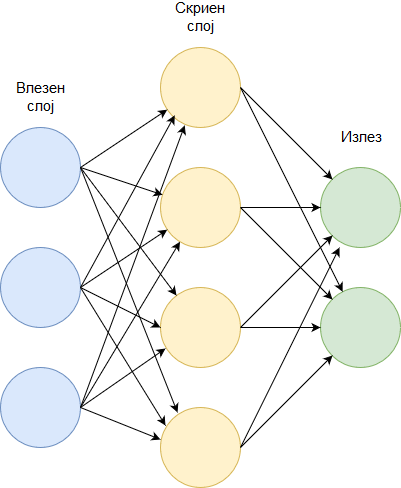
\includegraphics[scale=0.66]{images/nn.png}
	\caption{Елементарна длабока невронска мрежа}
	\label{fig:nn}
\end{figure}

\begin{figure}[H]
	\centering
    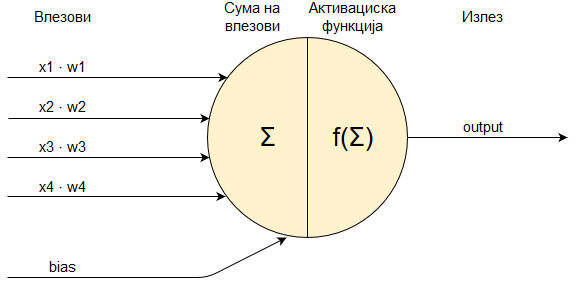
\includegraphics[scale=0.6]{images/nn_cell.png}
	\caption{Јазол од feed-forward невронска мрежа}
	\label{fig:ff_node}
\end{figure}


\section{Рекурентни невронски мрежи}

Рекурентните невронски мрежи се варијанта на Feed-forward мрежите со внатрешна меморија (или состојба) што ги оспособува за работа со секвенцијални податоци. Кај нив излезите од тековниот временски чекор се користат како влезови при наредните временски чекори. Меморијата во невроните се имплементира со механизам на порта (или влез) за меморија и мрежата има контрола над мемориските порти. Постојат повеќе варијанти на рекурентни невронски мрежи како на пример: целосно рекурентни невронски мрежи, рекурзивни невронски мрежи, LSTM, GRU итн. На слика \ref{fig:rnn_folded} може да се види неврон од рекурентна невронска мрежа. Невронската мрежа од вакви неврони може да ја разгледаме логички во одвиткана форма, при што секој временски чекор што го обработува мрежата може да го гледаме како паралелна feed-forward невронска мрежа, а таквото одвиткување на еден неврон може да се види на слика \ref{fig:rnn_unfolded}.

\begin{figure}[H]
	\centering
	\caption{Рекурентна невронска мрежа.}
    \begin{subfigure}[t]{1\linewidth} 
        \centering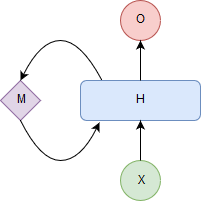
\includegraphics[width=.3\linewidth]{images/rnn_folded.png}
        \caption{Ќелија од рекурентна невронска мрежа. X е влезот, H внатрешната состојба, O излезот и M меморијата на ќелија од рекурентната невронска мрежа.}	
        \label{fig:rnn_folded}
    \end{subfigure}
    \begin{subfigure}[t]{1\linewidth}       
        \centering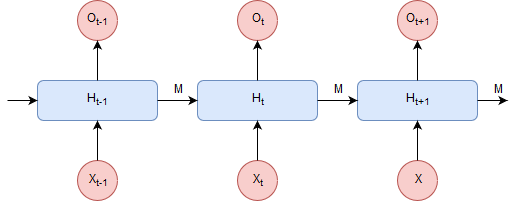
\includegraphics[width=.7\linewidth]{images/rnn_unfolded.png}
        \caption{Одвиткана претстава на рекурентна невронска мрежа. Одвиткан поглед на ќелијата од \ref{fig:rnn_folded}. Во временски момент $t$ ќелијата го прими својот излез од временски чекор $t-1$, а го зачувува за временскиот чекор $t+1$.}
        \label{fig:rnn_unfolded}
    \end{subfigure}
	\label{fig:rnn}
\end{figure}

\subsection{Back-Propagation Through Time}
Рекурентните невронски мрежи се тренираат со BPTT алгоритамот, со кој се ажурираат вредностите на тежиниските параметри на ќелиите. Алгоритмот може да се сумира со следните чекори:
\begin{itemize}
    \item Приказ на влезен примерок на мрежата и пресметка на излезите низ сите слоеви во мрежата.
    \item Споредба на добиениот излез од крајниот слој и саканиот излез и пресметка на грешка.
    \item Пресметка на градиенти на грешката во однос на тежинските параметри на мрежата.
    \item Промена на тежинските параметри на мрежата со цел намалување на пресметаната грешка.
    \item Повторување.
\end{itemize}

За секвенца со должина N временски чекори, RNN работат така што ја одвиткува мрежата за секој временски чекор, и за секој има еден влезен елемент и една копија од мрежата. Грешките се пресметуваат чекор по чекор, а потоа се пресметува кумулативна грешка за секвенцата и мрежата се замотува и се извршува промената на тежинските параметри со цел намалување на пресметаната кумулативна грешка. Пресметковната комплексност на алгоритамот расте со бројот на временски чекори во секвенците што се обработуваат. 

\subsection{Truncated Back-Propagation Through Time}

Поради директната зависност на пресметковната комплексност од дожините на секвенците што се обработуваат, не е практично да се тренира RNN модел со долги секвенци со BPTT алгоритамот. TBPTT алгоритамот е апроксимативна верзија на BPTT алгоритамот со кој се решава проблемот на пресметковна комплексност. Кај него секвенцата се обработува само чекор по чекор, при што ажурирањето на тежинските параметри се врши на секои k1 временски чекори, при што грешката се пресметува само за последните k2 временски чекори. Алгоритамот може да се сумира со следните чекори:
\begin{itemize}
    \item Приказ на секвенца од k1 број временски чекори и пресметка на нивните излези.
    \item Одвиткување на мрежата и пресметка на акумулирана грешка за k2 временски чекори наназад.
    \item Завиткување на мрежата и ажурирање на тежинските параметри.
    \item Повторување.
\end{itemize}

Со параметрите k1 и k2 ги дефинираме перформансите на мрежата. Со k1 се условува колку брзо ќе се тренира мрежата т.е. колку често ќе се ажурираат нејзините тежински параметри, а со k2 се условува колкав ќе биде прозорецот за гледање наназад во секвенцта, т.е. колку од секвенцата може да види при секој временски чекор мрежата. Поголема вредност за k2 овозможува повеќе можност за учење на глобална структура, меѓутоа со преголемо зголемување мрежата може да ги изгуби можностите за учење поради нулирање на градиентите на тежинските параметри.

\subsection{Експлодирачки / нулирачки градиент}

Голем проблем кај рекурерентните невронски мрежи претставуваат експлодирачкиот и нулирачкиот градиент. И двата проблеми доаѓаат од начинот на пресметка на грешка и ажурирање на тежините. Грешката се пресметува за секој временски чекор, а градиентите на грешка се мултиплицираат при чекорот на ажурирање. Доколку се појавува често вредност поголема од 1.0, вредностите на градиентот скокаат брзо и мрежата станува нестабилна. Ако има повеќе такви градиенти еден по друг акумулираната вредност може да стане и поголема од капацитетот за целобројни вредности на машината на која се извршува алгоритамот, што причинува overflow и NaN вредности. Оваа појава се нарекува експлодирачки градиент. Нулирачки градиент е пак спротивното кога вредностите на градиентот на грешка се премали, па тежинските параметри на одредени (или дури сите) ќелии во мрежата постануваат нула, што ефективно ги умртвува (или деактивира). Експлодирачкиот и нулирачкиот градиент влијаат на способноста на мрежата да учи долги секвенци. Еден од начините да се намали нивното влијание е да се ограничи бројот на чекори за ко    и се акумулира (пресметува) градиентот на грешка.

\section{Long Short-Term Memory}

Long Short-Term Memory - LSTM, е една од пософистицираните варијанти на ќелии за рекурентни невронски мрежи кои се обидуваат да го решат проблемот на експлодирачки/нулирачки градиент, која додатно има и можност за учење на произволно долги секвенци. Секоја LSTM ќелија има константна рекурентна врска, со тежински параметер константно поставен на 1.0. Ова врска и дава мемориски капацитет на ќелијата и овозможува константен пренос на градиентот на грешка, што ја штити ќелијата од нулирачки градиент. 
LSTM ќелиите имат 3 карактеристични порти кои го управуваат нивното работење: порта за заборавање, порта за модификација и порта за излез. Во одредени ситации е корисно ќелијата да го „заборави“ тоа што го има во својата меморија, како на пример кога содржи ирелевантни или застарени податоци. За таа цел LSTM ќелиите имаат влез за заборавање, кој што прима вредност од 0 или 1. Содржината на ќелијата се множи со таа вредност, па така кога е 0 ќелијата практично заборава се, а кога е 1 помни се, нема можност за парцијална модификација на вредноста. Наспроти ова, во ситуации кога содржината на ќелијата треба да биде заштитена од модификација во одреден временски чекор, се користи порта за модификација. Со неа може да се заштити содржината на ќелијата повеќе временски чекори, овозможувајќи користење на информации во тековниот временски чекор од пред произволем број временски чекори. Последната порта, портата за излез овозможува игнорирање на излезот од ќелијата. Ова е корисно во ситуации каде повеќе ќелии би имале релевантна информација, но некои од нив имаа хипотетички порелевантна информација, па тие што не се толку релевантни излезот им го игнорира мрежата со користење на портата за излез. Пример LSTM ќелија може да се види на слика \ref{fig:lstm}.

\begin{figure}[H]
	\centering
    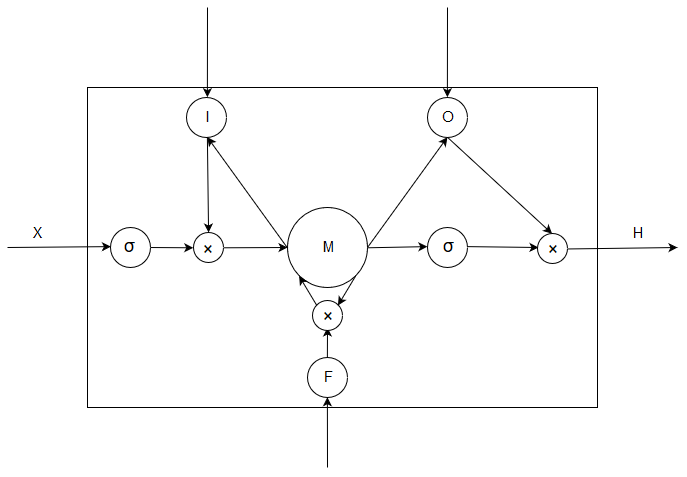
\includegraphics[scale=0.6]{images/lstm.png}
	\caption{LSTM ќелија}
	X го претставува влезот од тековниот временски чекор, M ја чува меморијата, I е порта за модификација, F е порта за заборавање, O е порта за излез, а H е излезот од ќелијата.
	\label{fig:lstm}
\end{figure}

Овие карактеристи ги прават мрежите изградени од LSTM ќелии способни за работа со доста долги секвенци, со должини поголеми и од 1000 елементи, како и со работа со секвенци со произволна должина, со секвенци во кои има доста шум, секвенци кои што не може едноставно да се компресираат итн.

\section{Вградување на зборови во латентен простор}

При работа со податочни множества каде што има голем број на уникатни влезни елементи, категоричната репрезентација на влезните елементи, т.н. 1-hot вектор (бинарен вектор со должина еднаква на бројот на уникатни влезни елементи, каде што само една позиција има вредност 1 а сите останати 0, а тоа е позицијата на влезниот елемент во подреденото множество на уникатни влезни елементи) има драстично влијание врз перформансите на моделите за машинско учење. Таквите вектори се екстремно ретки и причинуваат пресметко проблеми со денешните алатки за машинско учење, бидејќи ниедна нема ефикасна податочна репрезентација на ретки вектори и матрици. 
Едно практично решение на овој проблем претставува вградувањето во латентен простор. Елементите од оригиналното множество ги претставуваме со многу пократок вектор со фиксна должина. Овој вектор се состои само од реални вредности, и претставува компресирана и дистрибуирана репрезентација на оригиналниот влезен вектор. Овој вектор и процесот на вградување може да се изведе со невронски мрежи, а зависно од начинот на кој ќе се тренира мрежата, во него може да се вградат различни семантички информации за влезното множество. Големината на векторот на вградување обично се движи помеѓу десетици и стотици елементи.
Вградувањето може да се тренира одделно или како дел од главниот модел за машинско учење за кој е наменето. Одделното тренирање е добро доколку има потреба од повторно искористување на вградувањето кај други модели, бидејќи може да се зачува како независна компонента. Од друга страна ако не се планира користење надвор од моделот, тренирањето како елемент во моделот е поедноставно и попрактично.

Наједноставна имплементација на вградувањето во латентен простор е кога тоа е елемент во моделот. Се имплементира со користење на еден или повеќе feed-forward слоеви, чија големина и број се параметери на моделот, каде големината обично е во ранг на стотици елементи. Векторот се иницијализира со мали случајни броеви, а слоевите се тренираат со Backpropagation алгоритамот. Во трудот \cite{Sutskever2014} се искористени вакви слоеви за учење на секвенци од зборови. 

Word2Vec вградувањето, претставен во трудот \cite{Mikolov2013}, е пософистициран модел за вградување на зборови во латентен простор. Со користење на статистички методи за анализа на колокација на зборови во моделот се додава информации за поврзаноста помеѓу зборовите според тоа колку често се појавуваат заедно. Има две варијанти на моделот: bag-of-words и skip-gram. Првата варијанта ги учи вградувањата така што го предвидува тековниот збор врз основа на контекстот, додека другиот модел ги предвидува ближните зборови врз основа на тековниот. 
Chord2Vec моделот, од трудот \cite{Madjiheurem2016}, претставува имплементација на skipgram моделот од Word2Vec со NADE елементи. Наменет е да ги научи појавувањата на нотите во контекст на акорд, со цел генерирање на акорди како основен дел од музичка композиција. 

\section{Gibbs sampling / Гибсово семплирање}

Гибсово семплирање е техника за генерирање/избирање на примероци од мултиваријабилна дистрибуција каде што ни е познат само дел од условните дистрибуции. Техниката е Монте Карло Марков Ланец и се базира на претпоставката дека може да ги пресметаме условните дистрибуции на една од променливите условени од сите други променливи, и дека можеме да вадиме примероци од добиените дистрибуции. Гибсово семплирање е доста корисно за вадење на примероци од непозната дистрибуција. Има повеќе видови на имплементации како: блок \cite{Boulanger-Lewandowski2012, Goel2014}, случајно скенирање, псеудо \cite{Hadjeres2016}, со колапс и др. Според \cite{Hadjeres2016} техниката е погодна за модел за музика само доколку работиме со категорични податоци (1-hot вектори или симболи), а не со пијано ленти, бидејќи не може да се справи добро со симултано менување на повеќе променливи.

\chapter{Евалуација}
\label{ch:evaluacija}

Музикалноста на одредена секвенца од ноти или комбинации од ноти не може да се оцени објективно, т.е. не постои математичка фунцкија која може да се примени на секвенца со која ќе се добие конкретна вредност за нејзината музикалност, пријатност за слушање и "музички коректност". Поради тоа секој обид за креирање на систем за генерирање на музика со машинско учење се соочува со две големи пречки: немање на оптимизациска функција при учење и немање на начин за објективна оцена на квалитет на резултатите и компарација на моделите. 
Првиот проблем увиден во поголемиот дел од трудовите разгледани во поглавје \ref{ch:pregled} (\cite{Tikhonov2017,Boulanger-Lewandowski2012,Boulanger-Lewandowski2014,Liang2017,Johnson2017,Yang2017,Eck2002,Goel2014}) авторите го имааат заобиколено така што ја оценуваат способноста на моделот да повторува секвенци, т.е. една секвенца е добра/музикална ако е иста/слична на веќе постоечка. Објективна функција за оптимизација на моделите која ја користат е одредена варијанта на крос-ентропија, бинарна или категорична. Постојат и историски примери каде што објективната функција за оптимизација е човек оценувач \cite{Biles1994}, меѓутоа воопшто не се практични во модерни системи со масивно паралелни пресметки.
Финалните резултати од системот може единствено да се оценат на субјективен начин. Најчесто тоа се прави со некоја форма на анкетирање, интервјуа или тестови. На пример во трудот \cite{Hadjeres2016} каде што се генерирани корали во стилот на Јохан Себастијан Бах, добиените корали се оценети споредувајќи ги со оригинални корали од Бах. Оценувањето е направено од страна на 1272 луѓе со различно ниво на познавање на класична музика и музичка теорија. На оценувачите им биле презентирани колекција од композиции, мешавина од оригинални композиции и генерирани композиции, една по една, и им била дадена бинарна опција да изберат дали дадена композиција е оригинал или генерирана.
Во трудот \cite{Liang2017}, во кој што исто се генерирани корали од Бах, оценувањето е направено на сличен начин како во \cite{Hadjeres2016}, со тоа што било анкетата била објавена на социјалните мрежи, и корисниците биле идентификувани по IP адреса. Тие првично биле испрашани за старостна група и познавања на музика. Потоа следувале 5 прашања, т.е. 5 парови од генерирана и оригинална музика. Првите 2 прашања содржат целосно генерирана композиција, а останатите 3 содржат делумно генерирана композиција или хармонизација. Анкетираните требале да одредат која композиција од секој пар е оригинална а која е генерирана.
Овој тип на оценување е сличен на Турингов тест. На сличен начин, оценување може да се направи со рангирање на резултатите. Во трудот \cite{Yang2017} е опишано рангирање на добиените резултати од нивниот кандидат алгоритам и резултати од други алгоритми претходно искористени на истото податочно множество. На 21 оценувачи, кои примарно се занимавале со компјутерски науки, со различно, но не-професионално, познавање на музика и музичка теорија, им биле презентирани резултати добиени од две варијанти на MidiNet моделот и едена варијанта на MelodyRNN моделот. На оценувачите им било кажано дека некои од примероците се реална музика, иако сите примероци биле генерирани, и нив ги оцениле со оценка од 1 до 5 според Ликертова скала.
Поедноставен пример со рангирање може да се види во \cite{GarciaSalas2011}, каде што на 30 учесници од различна возраст и познавање на музика, од кои поголем дел биле од ИТ индустријата, им биле пуштени 10 песни, 5 генерирани од човек, а 5 од алгоритмот, и нив ги рангирале по тоа колку им се допаѓаат.

\chapter{Податоци}
\label{ch:podatoci}

Огромно количество на музика е достапно на интернет во многу различни формати. Најосновна поделба на достапната музика е на интерпретирана и симболична. Интерпретирана музика е било каква снимка на музика во конкретна изведба, запишана во датотека како сиров или компресирани аудио запис, со или без загуба на квалитет, на пр: .wav, .mp3, .m4a, .flac датотеки. Симболична музика е рачно запишана и е слободна за интерпретација, т.е. не се репродуцира директно. Таа е достапана во многу разноврстни формати, со различен степен на интерпретабилност, како на пр: ABC, MIDI, петтолиние, текстуални табулатури, акордни секвенци.
Работањето со интерпретирана и симболична музика носи сосема различни предизвици. Во овој труд ќе работам исклучиво со симболична музика, па во продолжение ќе ги разгледам особеностите на симболичната музика и работење со неа во контекст на машинско учење.

\section{Податочна репрезентација}

Симболичната музика доаѓа во разноврстни изворни формати, со различен степен на машинска интерпретабилност и погодност за користење во системи за машинско учење. Најпогодни изворни формати се MIDI форматот и разните текстуални формати како на пр: акордни записи, ABC записи и табулатури. 

\subsection{Изворни формати}

\subsubsection{MIDI}

MIDI е индустриски стандард за протоколи, дигитални интерфејси и конектори за дигитални музички инструменти и гарантира интероперабилност помеѓу инструментите, софтверска опрема и дигитални додатоци за инструменти. MIDI датотеките се користат за дигитална репродукција на музика, и се многу покомпактни од било каков снимен музички запис, но немаат капацитет за репродукција на човечки глас. При репродукција недостасува добар дел од финесите при изведба на музиката кои ја прават интересна.

Датотеките се структурирани како секвенци од MIDI пораки кои носат информации за: отсвирени ноти (почеток, крај, интензитет, тон), контролни пораки (волумен, ефекти, клок сигнал) и пораки со мета-информации. Најзначајни се пораките за почеток и крај на свирење на одредена нота:
\begin{itemize}
    \item \texttt{Note\_on} настан означува почеток на свирење на одредена нота. Има 3 параметри: каналот во кој треба да се отсвири нотата, висината на тонот што треба да се отсвири (помеѓу 0 и 127 според MIDI стандардот) и брзина со кој треба да се отсвири. На пр: <\texttt{Note\_on}, 0, 60, 50> настанот носи информација дека треба да се отсвири нота со висина 60 т.е. C4, во првиот канал со брзина 50.
    \item \texttt{Note\_off} настан означува прекин на свирење на одредена нота. Има ист формат како \texttt{Note\_on} настанот. На пр: <\texttt{Note\_off}, 0, 60, 20> настанот означува прекин на свирење на гореопишаната нота, со таа разлика што престанувањето би било со брзина 20.
\end{itemize}
Овие настани не носат информација за време, па затоа се вградени во делови од трака (анг. track chunks) во кои се содржат сите потребни временски информации. Овие информации се запишани во тн. делта време, кое може да биде изразено во секунди или во метрички единици (фракции од времетрање на цела нота).
Овие пораки може да се искористи директно во модел за машинско учење со едноставна енумерација на сите можни вакви пораки пронајдени во податочното множество. Меѓутоа ова не е иделано решение бидејќи така моделот би немал никаква индикација дека две пораки ја претставуваат истата нота ако дел од параметрите се разликуваат само за малку (на пр. во брзината), и би немал никаква информација за истовремено свирење на нотите.

\subsubsection{Текстуални формати}

Текстуалните формати се идеални кандидати за обработка со користење на техники за обработка на природни јазици. Тие се состојат од секвенца на акорди или мелодиска линија и пропратен текст доколку песната има текст. Успешен систем за генерирање на музика со користење на ABC форматот, кој е популарен формат за запишување на народна музика, може да се види во трудот \cite{Sturm2015}. Пример за песна запишана во текстуален формат, поточно акорден запис може да се види на слика \ref{fig:akordi}, извадок од „Ода на радоста“. Еден недостаток на овој тип на музички записи, во контекст на машинско учење, е интерпретабилноста, т.е. многу голем дел од деталите на изведбата не се забележи во записите. Тие се наменети за луѓе кои ја познаваат песната, да им даде упатства при изведба и полесно да може да ја научат песната. Два изведувачи, кои не ја познаваат најдобро конретната песна, може да ја изведат на сосема различни начини, пр. со различно темпо, различна метричка структура, различни времетраења на сегменти од песната итн. Поради тоа и тешко е да се оценат перформансите на систем кој би работел со датотеки во тесктутален формат, па објективно може да ги оценуваме како системи за генерирање на текст.

\begin{figure}[H]
	\centering
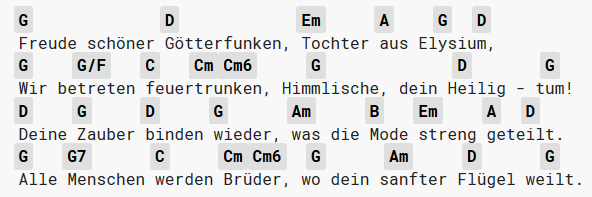
\includegraphics[scale=0.9]{images/ode_to_joy.png}
	\caption{Акорден запис}
	\label{fig:akordi}
\end{figure}

\subsection{Аспекти на податочна репрезентација за моделите за машинско учење}

Начинот на кој се трансформира изворниот формат на музиката во формат погоден за моделите за машинско учење драстично влијае на генеративните перформанси на моделот. Мали промени во податочната репрезентација може да доведат до израз различни музички особености во процесите на генерализација и генерирање на музика. Во продолжение се разгледани клучните аспекти на податочната репрезентација кои може да влијаат на модел за машинско учење за генерирање на музика.

\subsubsection{Репрезентација на времето}

Времето може да одлучиме да се претстави како основен елемент на податочната репрезентација, т.е. да се подели музиката во временски исечоци, или да се вгради како параметар на основните елементи на музичката секвенца, слично како што е тоа направено во MIDI датотеките. Првиот случај е многу почест, скоро исклучиво искористен во претходните трудови \cite{Hadjeres2016,Boulanger-Lewandowski2012,Boulanger-Lewandowski2014,Eck2002,Eck2008,Walder2016,Dong2017,Dong2018}. Предностите му се што е едноставен за креирање на податочен енкодинг и недвосмислена претстава на времето како и поедноставен приказ на акорди и полифонија. Недостатоци се реткоста (sparsity) на добиените примероци и честото повторување на идентични елементи во секвенците. На нив драстично влијае грануларноста (резолуцијата) на претставената секвенца. 

Претставање на времето како дел од елементите на музичката секвенца овозможува многу голема флексибилност, меѓутоа има доста недостатоци како на пр: нема ефикасен начен за енкодирање на времето во елементите, драстично го зголемува лексиконот на податочното множество, многу е комплексно да се енкодираат промени во тековно отсвирени ноти (пр. при промена на акорди, каде дел од нотите би останале активни, дел би престанале да се свират, а нови би биле активирани). Се ова влијае драстично на перформансите на хипотетички модел за генерирање на музика.

\subsubsection{Краеви на нотите}

При репрезентација на музиката со временски исечоци не постои разлика помеѓу две исти ноти отсвирени во два последователни исечоци и една нота со времетраење еднаква на сумата од времетраењето на двете поединечни ноти. Проблемот може да се пристапи на 3 начини:
\begin{itemize}
    \item Да се игнорира.
    \item Да се дуплира резолуцијата/грануларноста на податочната репрезентација од најмалото времетраење кое го има во податоците (или произволно одредено времетраење) со што ќе се додаде симбол за крај на ноти кој би се користел во секој друг временски чекор.
    \item Да се дуплира лексиконот на влезното множество, со што за секоја нота ќе има 2 симболи, еден за почеток еден за продолжување на нотата.
\end{itemize}
Вториот и третиот пристап го решаваат проблемот, меѓутоа ја дуплираат пресметковната комплексност на проблемот на учење и генерирање на музика.

\subsubsection{Резолуција}

При репрезентација на музиката со временски исечоци клучен фактор кој влијае на перформансите е резолуцијата/грануларноста на репрезентација на музичката секвенца. Поголема грануларност овозможува репрезентирање на поинтересни, брзи, покомплексни мелодии, меѓутоа резултира во поголеми мемориски побарувања на моделот за учење. Додатно зголемување на грануларноста резултира и во поголем број на празни елементи, а нотите со подолго времетраење ќе се повторуваат. Најчесто се одбира грануларност еднаква на најмалото времетраење на нота во податочното множество, меѓуто тоа не секогаш е идеално решение. Доколку релативно мал дел од елементите во податочното множество го имаат најмалото времетраење, може да се избере поголемо времетрање со цел подобрување на перформансите на моделот.

\subsection{Пијано лента}

Пијано лента е најчесто искористената податочна репрезентација за работење со музика со модели за машинско учење \cite{Hadjeres2016,Boulanger-Lewandowski2012,Boulanger-Lewandowski2014,Eck2002,Eck2008,Walder2016,Dong2017,Dong2018}. Музиката е поеделена на временски чекори, кадешто секој елемент претставува временски исечок со должина од дел од цела нота, или дел од секунда. Секој временски чекор ги претставува тековно исвирените ноти. Најчесто е бинарен вектор, кадешто секој елемент од векторот претставува одредена нота, според апсолутната вредност на висина на тонот (најчесто преку користење на pitch вредностите на нотите од MIDI стандардот), при што ненулта вредност означува дека таа нота се свири во моментот. Во одредени варијанти векторот е целоброен, и ненултите вредности опишуваат некоја особина на отсвирената нота како гласност или интензитет. Инспирирана е од старите пијано ленти од перфорирана хартија користени во само-свиречки пијана или метални ленти од музички кутии. На слика \ref{fig:piano_pr} може да се види реална пијано лента во самосвиречко пијано, а на слика \ref{fig:piano_roll} репрезентација на бинарна пијано лента.

\begin{figure}[H]
	\centering
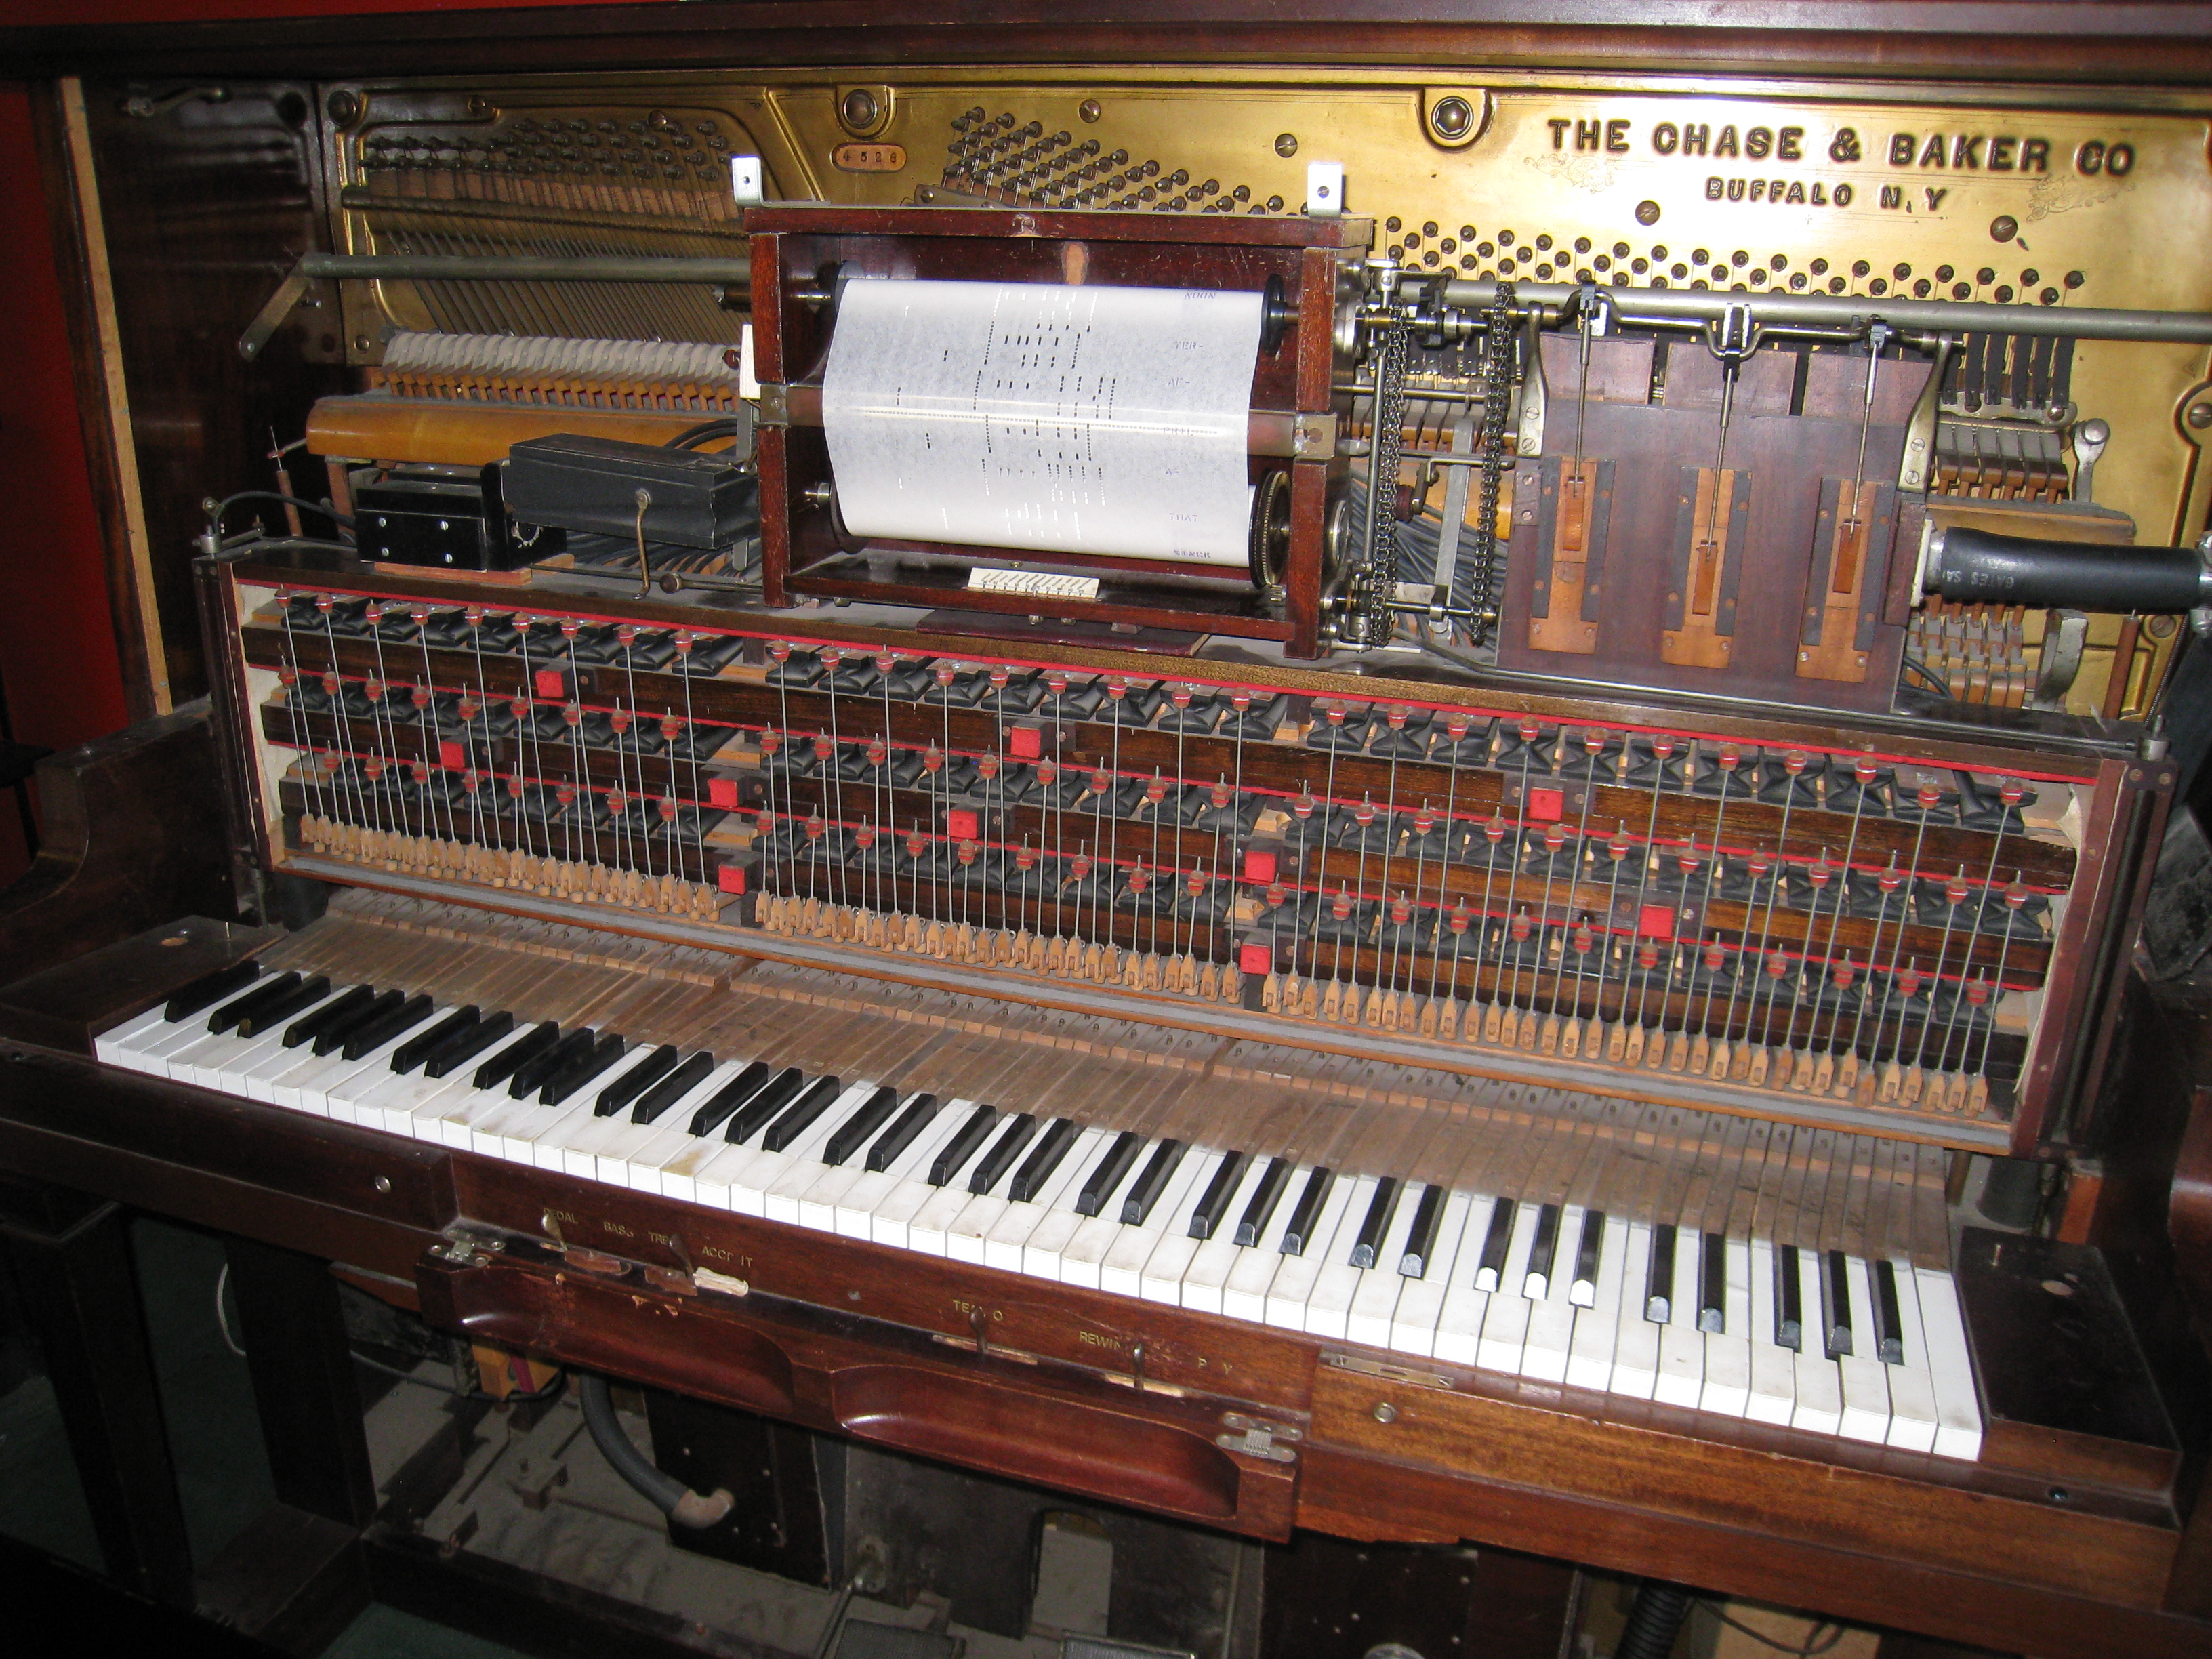
\includegraphics[scale=.3]{images/piano.jpeg}
	\caption{Самосвиречко пијано со пијано лента}
	\label{fig:piano_pr}
\end{figure}

\begin{figure}[H]
	\centering
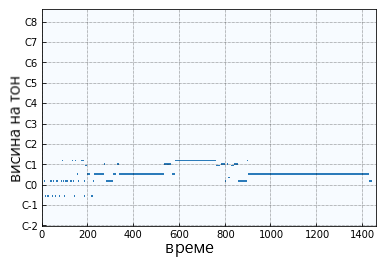
\includegraphics[scale=1.3]{images/piano_roll.png}
	\caption{Пијан лента}
	Хоризонталната оска го претставува времето, а вертикалната нотите според MIDI висини на тон
	\label{fig:piano_roll}
\end{figure}

\section{Предпроцесирање}

По одбирање на податочно множество и репрезентација на истото за подобрување на перформансите на моделот за машинско учење може да се изврши одредено предпроцесирање на податоците пред извршување на алгоритамо за машинско учење. Филтрирање на податочно множество, т.е. отстранување на песни користејќи одреден сет на критериуми за конзистентност може да помогне во подобрување на перформансите на системот. Критериумите можат да бидант на пр:
\begin{itemize}
    \item Сите песни да се напишани во конкретен клуч.
    \item Сите песни да се со одредена метрика.
    \item Сите песни да имаат темпо во одреден опсег.
    \item Да нема промена на метрика во песната.
    \item Песните да се комплетни и да нема оштетени или тешки за парсирање или пак двосмислени елементи.
    \item Нотите да припаѓаат само во одреден тонален опсег.
\end{itemize}

Додатно филтрирање може да биде извршено и во рамките на песните. Елементи од изворните податоци кои не носат експлицитно музички податоци обично може да се отстранат без последици. Одредени музички елементи кои вршат модификации на музичките елементи може да се отстранат со последицата дека се губат одредени нијанси на отсвирената музика. Информацијата за интензитет/гласност на отсвирена нота може исто така да се отстрани со мала загуба на детали. Доколку има ноти со помало времетраење од минималното избрано времетрање, тогаш пократките ноти може да се отстранат или продолжат. Доколку се работи во ограничен тонален опсег, нотите кои се надвор од опсегот може да се отстранат или транспонираат во тоналниот опсег.

\subsection{Транспозиција}

Транспозиција е техника за поместување на множество од ноти за одреден број на полутонови нагоре или надоле со константен интервал. Може да се изврши врз колекција од песни за збогатување на податочното множество. Поместувајки ги сите мелодиски линии во податочното множество во сите можни позиции во тоналниот опсег му овозможува тонална (или транслациона) инваријанса инваријанса на моделот за машинско учење и придонесува кон намалување на реткоста (sparsity) на влезните податоци. Транспозицијата може да се изврши на сите песни кон еден заеднчики основен клуч (\cite{Sturm2016,Tikhonov2017}) или на сите песни кон повеќе (потенцијално сите можни) основни клучеви (\cite{Yang2017,Bretan2016}).

\chapter{Алатки}
\label{ch:alatki}

Во продолжение е дадам краток опис на алатките кои се искористив за изработка на трудот.

\section{Keras}

Keras е библиотека за работа со длабоки невронски мрежи на високо ниво. Напишана е во Python програмскиот јазик и дава можност за работа со користење на една од трите најпопуларни библиотеки за машинско учење на ниско ниво: TensorFlow, CNTK или Theano. Приоритет на библиотеката е овозможување на брзо и едноставно креирање на прототипи на системи со машинско учење, и е едноставна за разбирање и користење. Паралелно процесирачките способности може да се користат на процесор или графички акцелератор. Библиотеката е екстремно модуларна, скоро сите елементи во невронските мрежи се конфигурабилни модули и лесно може да се менуваат. Истите модули се отворени и може да бида проширени или заменети од корисничка страна.

\section{Music21}

Music21 е Python библиотека за музикологија, развиена на MIT. Намета е да овозможни лесна и детална анализа на музички композиции во симболична форма. Покрај повеќе видови музички анализи, овозможува и модифицирање на музички датотеки, како и програматско креирање на музика и музички примероци. Поддржува низа на формати, од кои најзначајни се MIDI и musicxml. Покрај тоа содржи и повеќе колекции на класична музика од јавен домен кои може да се искористат за анализа или за тренирање на модели за генерирање на музика. 

\section{pypianoroll}

Pypianoroll е Python библиотека за работа со пијано лента записи. Подржува работа со записи со една или повеќе ленти, како и можности за транспозиција на постоечки пијано ленти. Овозможува и конверзија на MIDI датотеки во пијано лента и обратно, како и графичка визуелизација на пијано лентите.

\chapter{Студија на случај}
\label{ch:studija}

\section{Податочно множество}

Најдостапни и најлесни за компјутерска обработка извори на симболична музука претставуваат датотеките во MIDI формат. Во иницијалните фази на изработка беше искористено мало податочно множество коешто беше изградено од GuitarPro датотеки, рачно избрани од http://ultimate-guitar.com. Датотеките преставуваат кориснички генерирана репрезентација на музиката, примарно наменети за учење. Бидејќи системот за репродукција на звук за GuitarPro датотеките е базиран на MIDI стандардот, лесно може да се конвертираат во MIDI датотеки. Финалниот чекор за подготовка на податоците е трансформација во пијано лента репрезентација. За жал процесот резултираше во неквалитетна конверзија, песните во финалната форма имаа многу аномалии, неправилности и бесмислени елементи. Се појавија многу тонови со времетраење од 0 рамки (при конверзија на пиано лентата назад во MIDI датотека), како и тонови со времетраење од десетици секунди. Исто така се појави и истровремено свирење на 10 и повеќе тонови на гитара, што е невозможно со стандардна гитара. Добар дел од проблемите се резултат на нестандардниот квалитет на кориснички генерираните датотеки и на алатките за конверзија. Затоа беше одлучено да не се користат ваквите датотеки туку постоечко податочно множество.

\subsection{Лахк (Lahk) MIDI}

Лахк MIDI податочното множество се состои од 176.581 уникатни MIDI датотеки, собрани од страна на К. Рафел за целите на трудот \cite{Raffel2016}, во кој е претставен систем за пребарување и споредување на музички секвенци, или исечоци, од MIDI датотеки. Дел од ова множеството, наречен LMD-Matched, се состои од 45.129 датотеки спарени со соодветни метаподатоци од податочното множество MillionSongs, што овозможува пребарување, групирање и селекција по одредени критериуми како на пр. жанр, автор, стил, темпо итн. 
Врз основа на LMD-Matched податочното множество, Х. Донг за потребите на трудот \cite{Dong2017} го има конвертирано целото Лахк MIDI податочно множество во датотеки со пијано лента репрезентација. На веб страната на која е прикажан трудот се достапни повеќе верзии од множеството, и тоа:

\begin{itemize}
    \item LPD-Cleansed - Претставува прочистена верзија на податочното множество според следните критериуми: отстранети песни кои не се во 4/4 ритам, отстранети песни со повеќе од една промена на темпо, отстранети песни каде што првиот такт не почнува од рамка со индекс нула, задржани песните коишто со наголема сигурност се совпаѓаат со ставка од MillionSongs множеството.
    \item LPD-5 - Сите можни инстанци на инструменти во MIDI датотеките се групирани во следните 5 категории: тапани, пијано, гитара, бас и жичана секција; според MIDI програмскиот број на инструментот. Инструментите кои не припаѓаат на ниту една од овие категории се групирани во жичаната секција, со исклучок на синтисајзер, перкусии и звучни ефекти.
    \item LPD-17 - Слично на претходното множество со тоа што инструментите се групирани во 17 категории: тапани, пијано, хроматски перкусии, оргуља, гитара, бас, жичана секција, ансамбл, метални дувачки инструменти, дрвени дувачки инструменти, писка, главен синтисајзер, придружен синтисајзер, народни инструменти, перкусии и звучни ефекти.
\end{itemize}

LPD-5 податочното множество се покажа како одлична појдовна точка за изградба на помало податочно множество за експериментите, бидејќи содржи песни со константен 4/4 ритам. Сепак потребна е додатна модификација за да биде пригодно за употреба. Не сите песни ги имаат сите инструменти, а некои песни имаат повеќе инструменти групирани во една трака, поради што потребна беше додатна обработка и селекција за да се добие квалитетно податочно множество.

\section{Податочна репрезентација}

Песните во LPD-5 податочното множество се во пијано лента репрезентација, каде што времето е поделено така да една рамка од лентата претставува 1/24 од еден удар, што за 4/4 ритам значи должина на такт од 96 рамки. Една рамка се содржи од 128 целобројни вредности, по една за секоја од можните ноти или звуци опишани со MIDI стандардот, при што вредноста го опишува интензитетот со кој е присутен звукот. Ваквиот вектор не е соодветен како елемент на модел за учење на секвенци, бидејќи таквиот модел би решавал паралелно 128 проблеми на регресија. Затоа првиот чекор во прилагодување на векторот претставува неговата бинаризација, т.е. во секоја рамка, секоја ненулта вредност се заменува со единица. Во обратна насока, при дебинаризација на векторот, единиците се заменуваат со рачно одредена вредност за интензитет, односно 2/3 од максималната вреднос. На овој начин се губи експресивност и нијанса при изведба на музиката, меѓутоа драстично се олеснува проблемот на учење на секвенците. 
По иницијалните експерименти во коишто беше трениран модел на секвенци од тн. "multi-hot" вектори (бинарни вектори кадешто повеќе вредности може да бидат активни истовремено), како што е бинаризираната варијанта на пијано ленти, беше увидено дека ваквите секвенци претставуваат тежок проблем за учење. Учење на 128 паралелни бинарни класификации резултираше во многу ретки активации на излезниот слој, а во рамките кадешто се појавија повеќе активации, комбинациите на ноти често беа бесмислени. Ова доведе до идеја за изградба на лексикон од сите можни комбинации на ноти, и користење на елементите од лексиконот како влез во моделот за учење. Трансформацијата е извршена така што 128 елементниот вектор се семета како 128 битна бинарна репрезентација на цел број. Лексиконот е изграден од ваквите целобројни репрезентации со додатни симболи за почеток и крај на песна/секвенца т.е. START и END и HOLD симбол за заддржување повторување на претходната временска рамка. Лексиконот потоа се индексира и секој елемент доаѓа на влез на моделот во "one-hot" или 1-n бинарен вектор. Во ваквиот вектор сите вредности се нула, освен вредноста со ист индекс како индексот на елементот во лексиконот, којашто е единица.

\section{Селекција на песни}

Датотеките од податочното множество содржат 5 ленти кои ги претставуваат инструментите: тапани, пијано, гитара, бас и жичана секција. Меѓутоа не сите датотеки имаат податоци во сите ленти. Бидејќи во жичана секција се групирана многу инструменти, што често може да доведе и до групирање на повеќе ленти од изворната датотека во една, беа филтрирани сите датотеки што содржат податоци на таа ленти. Голем број на песните не ја содржат пијано лентата, па бидејки примарна цел е генерирање на рок песни коишто најчесто немаат пијано делови, беа филтрирани и песните што содржат пијано. Останатите песни беа филтрирани така да лентите за тапани, гитара и бас гитара се целосно исполнети. Од добиеното подмножество со случајна селекција беа избрани 500 песни, од коишто поголем дел природно се погодија од рок, поп-рок и метал жанр. Од ова подмножество беа креирани MIDI датотеки со користење на pypianoroll библиотеката. Потоа со рачна инспекција беа избрани 50 песни според субјективна процена за квалитетот на добиената датотека, познавање на песната, жанровска припадност и релативна едноставност на песната.

\section{Транскрипција на песните}

За збогатување на податочното множество и гарантирање на транслациона инваријанса на мелодиските линии беше искористена постапка на музичка транскрипција. Иницијално беше извршена транскрипција на сите песни кон сите можни основни клучеви. Прво беа одредени најнискиот и највисокиот тон присутен во избраното податочно множество. Потоа за секоја од песните беше извршена транскрипција надолу за толку полутонови колку што има од најнискиот тон во податочното множество и најнискиот тон во самата песна, и нагоре за толку полутонови колку што има помеѓу највисокиот тон во податочното множество и највисокиот тон во поесната. Ваквата стратегија резултираше во различен број на транскрипции по песна, зависно од колку голем е тоналниот опсег на песната, што значи некои песни се поприсутни во резултантното транскрибирано податочно множество, а некои помалку присутни; но и во најголем можен број на транскрипции. Транскрипцијата беше извршена само на траките за гитара и бас, бидејќи нема смисла за тапани, таму MIDI пораките го немаат истото значење како кај останатите инструменти. Ваквата транскрипција резултираше во преголем број на можни влезни елементи, дури со 10 или повеќе оригинални песни, се добиваа повеќе од 15 транскрипции по песна, како и многу голем број на комбинации на ноти коишто многу ретко се среќаваат во реални песни. Бројот на влезни елементи во таквото множество беше толку голем, да не беше возможно да се извршува моделот на постоечкиот хардвер. Поради тоа мораше да се напушти ваквиот пристап на транскрипција. 

Со транскрипцијата на сите песни кон заеднички клуч се постигнува добар дел од посакуваните ефекти како со транскрипција кон сите можни клучеви. Недостатокот е што сите песни се центритрани на одреден тонален оспег, и можно е да има потреба генерираните песни да се поместат кон друг клуч рачно за да бидат во најсоодветниот тонален опсег за нив. Потенцијална придобивка од ваквата транскрипција е намалување на бројот на влезни елементи, што би го олеснило проблемот на учење на секвенци. Извршена беше транскрипција кон основен клуч $C4$ или MIDI тон 60.

\section{Архитектура за учење}

Архитектурата е имплементирана со користење на Keras библиотеката за длабоко учење. Моделот за учење се состои 3 подмодели, по еден за секој од инструментите. Подмоделите меѓусебе се идентични. Архитектурата за еден од подмоделите, на пр. гитара, е претставена на цртежот \ref{fig:architecture}. Една влезна рамка за секој од подмоделите се состои од 3 вектори кои ја претставуваат тековно отсвирената комбинација на ноти за конкретниот инструмент во временскиот момент кој го претставува рамката. Моделите започнуваат со 3 влезни блока, еден блок кој на влез прима N временски рамки од тековниот временски момент наназад, еден блок на влез ја примат тековната временска рамка, а последниот модел прима N временски рамки нанапред, каде N е параметар за одредување на способноста на моделот да гледа кон назад и напред во времето.

Секој од влезните блоковите има излез во тн. блок за вградување кој претставува тесно грло, и има помал број на јазлик од претходниот влезен слој. Задачата на овие блокови е да извршат компресија на податоците. По слоeвите за вградување следуваат блоковите за учење, 2 LSTM блока и еден целосно поврзан блок. Излезите од блоковите за вградување одговорни за секвенците од временски рамки за минатото и за иднината, одат во LSTM блковите, додека излезот од блокот за вградување на тековната рамка оди во целосно поврзаниот блок. LSTM блоковите ги учат временските зависности за соодветниот инструмент врз основа на временските рамки од минатото и од иднината, додека целосно поврзаната мрежа ги учи зависностите на тековно отсвиреното од соодветниот инструмент и останатите инструменти во даден временски момент. 

Излезите од LSTM блоковите и целосно поврзаниот блок се агрегираат во влезен вектор за финалниот целосно поврзан блок, чија задача е да ја учи, и подоцна предвиди, тековно отсвирената комбинација ноти за соодветионит инструмент.

\begin{figure}[H]
	\centering
    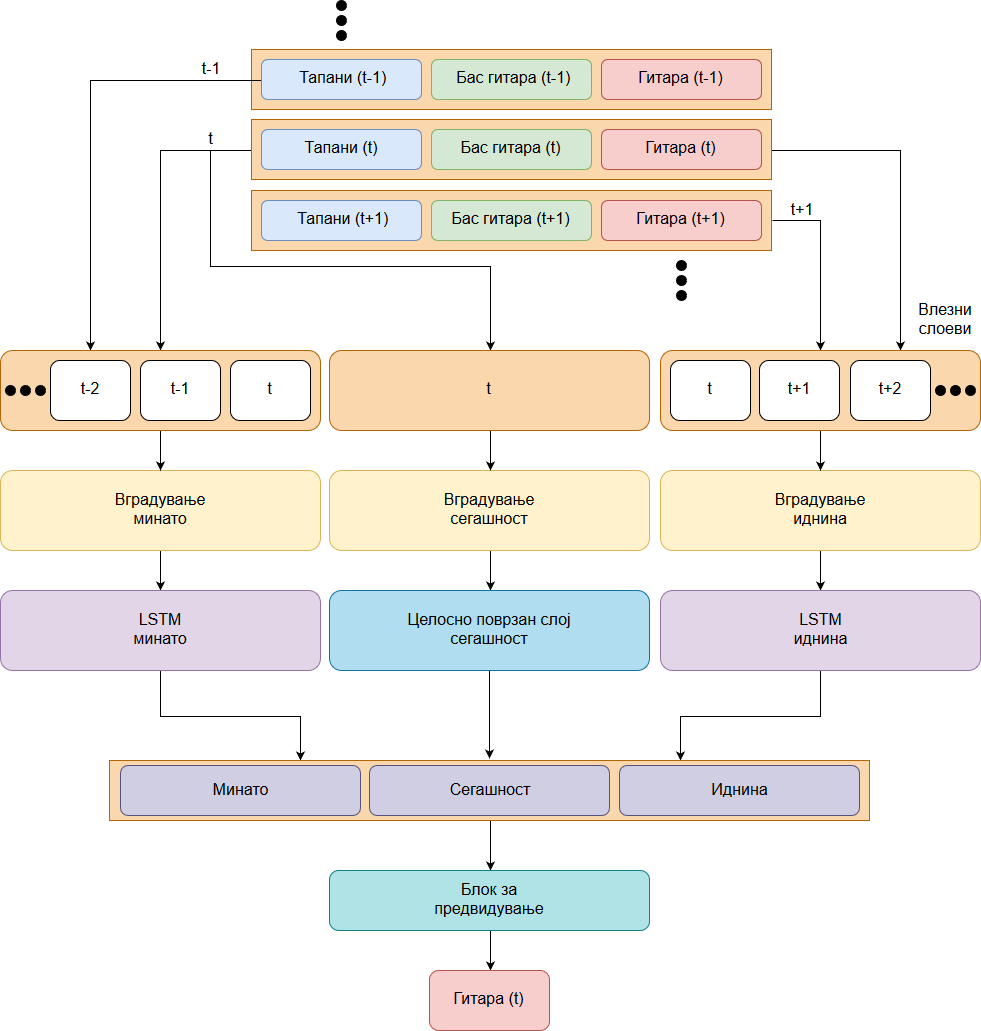
\includegraphics[scale=0.42]{images/arch.png}
	\caption{Архитектура на модел за учење.}
	Модел за учење на музички секвенци од гитара, во контекст на песна со 3 инструменти: тапани, бас гитара и гитара
	\label{fig:architecture}
\end{figure}


\subsection{Блокови за вградување}

Блоковите за вградување се изградени како целосно поврзана невронска мрежа со еден слој од 256 јазли. Влезната димензија на слојот е еднаква на големината на лексиконот, а излезот е реално вредностен вектор од 256 елементи. Ваквиот блок е прикажан на слика \ref{fig:embedding}.

\begin{figure}[H]
	\centering
    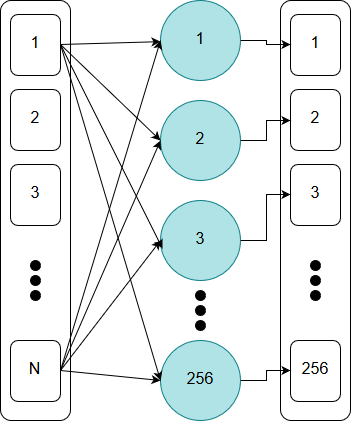
\includegraphics[scale=0.5]{images/embedding_block.png}
	\caption{Блок за вградување.}
	N е големината на влезниот вектор, а излезниот вектор има големина еднаква на бројот на јазли во мрежата (256)
	\label{fig:embedding}
\end{figure}

\subsection{LSTM блок за учење на секвенци}

Двата LSTM блока се составени од два слоја по 256 LSTM јазли. Влезната димензија е еднаква на излезот од слојот за вградување (256) помножен со бројот на временски чекори кој се гледа наназад, или нанапред (48), познат како lookback, а излезот е реалновредностен вектор со 256 елементи, со активациска функција тангенс хиперболикус. Излезите ги претставуваат предвидувањата за тековниот чекор врз основа на временскиот сегмент што го надгледува конкретниот блок. Бројот на временски чекори кој се гледа наназад и или нанапред доаѓа на игра во TBPTT алгоритамот, кој што во Keras ја одредува големината на подсеквенцата од временски чекори коишто и се даваат на LSTM подмрежата во одреден момент и бројот на чекори на кои се врши ажурирање на тежинските параметри, т.е. $k1=k2$. 
Ваков блок е прикажан на слика \ref{fig:lstm_block}

\begin{figure}[H]
	\centering
    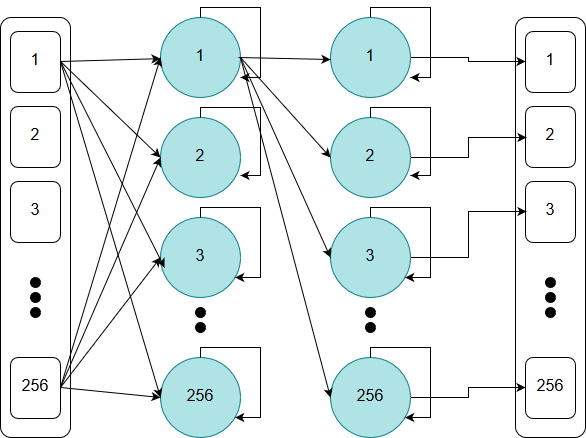
\includegraphics[scale=0.5]{images/lstm_block.png}
	\caption{Блок за учење на секвенци.}
	\label{fig:lstm_block}
\end{figure}

\subsection{Целосно поврзан блок за тековната временска рамка}

Овој блок е изграден од еден целосно поврзан слој од 256 јазли. Влезната димензија е еднаква со големината на излезот од слојот за вградување, а излезот е реално вредностен вектор од 256 елементи, со ReLU (Rectified Linear Unit) активација. Овој блок е прикажан на слика \ref{fig:fully_connected_block}

\begin{figure}[H]
	\centering
    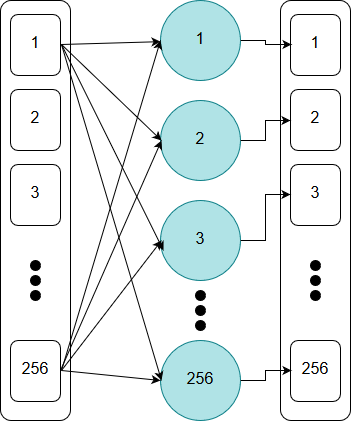
\includegraphics[scale=0.5]{images/fully_connected.png}
	\caption{Целосно поврзан блок за тековна временска рамка.}
	\label{fig:fully_connected_block}
\end{figure}

\subsection{Блок за предвиување}

Излезите/предвидувањата од двата LSTM блока и целосно поврзаниот блок се соединуваат во еден поголем вектор кој служи како влез во финалниот блок за предвидување. Овој блок е составен од целосно поврзан слој со број на јазли еднаков на големината на лексиконот. Влезната димензија е еднаква на збирот од излезните димензии на претходните блокови за предвидување ($3*256=768$), а излезот е бинарен вектор со димензија еднаква на големината на лексиконот, со softmax активација. Излезот од овој блок го претставува предвидувањето за вредноста отсвирена од конкретниот инструмент претставен со моделот, во тековниот временски чекор. На слика \ref{fig:learner} е прикажан блокот за предвидување.

\begin{figure}[H]
	\centering
    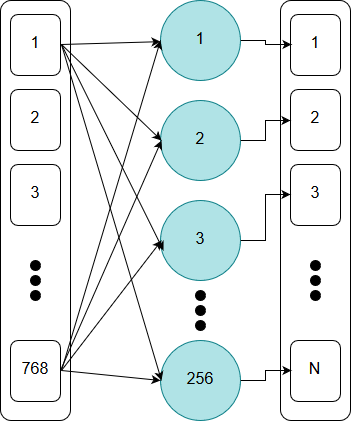
\includegraphics[scale=0.5]{images/learner.png}
	\caption{Целосно поврзан блок за предвидување на отсвирената временска рамка.}
	N е големината на лексиконот којшто служи за влез во системот.
	\label{fig:learner}
\end{figure}

\section{Тренирање на моделот}

Процесот на тренирање започнува со претворање на песните од пијано лента формат во секвенци од елементи од лексиконот. Лексиконите се состојат од: 567 елементи за тапани, 310 за бас гитара и 4499 за гитара, вклучувајќи ги симболите START, END и HOLD. На почетокот и крајот на песните прво се додаваат  START и END симболите, а потоа се додаваат HOLD симболите секаге каде што тековниот елемент е идентичен на претходниот. 

Од песните се градат влезно-излезни парови за моделите. Влезниот елемент е составен од три дела: прозорец со должина 48 рамки од $t-31$ временскиот момент до сегашната рамка, вклучително со неа; сегашната рамка; и прозорец со должина 48 рамки од сегашната рамка до $t+31$ временскиот момент, при што во временските рамки се соржат елементи за сите 3 инструмента. Излезниот елемент за секој од моделите се содржи од тековната рамка за соодветниот инструмент.

Секвенците од влезно-излезни парови од песните се комбинираат во една подолга секвенца. Од неа се формира python generator, што е структура за прелистување на произволно долги секвенци. Генераторот се состои од вкупно X примероци, поделени на 80\% за тренинг и 20\% за валидација. Моделите се тренираат еден по еден со користење на овој генератор во 50 епохи. Податоците се приложуваат на моделот во бечови од 128 елементи. Моделот се тренира со Adam оптимизаторот, оптимизира функција на загуба категорична крос-ентропија пресметана на предвидувањето за тековната рамка за соодветниот инструмент, и неа ја пресметува врз основа на метрика за прецизност на тренинг и валидациските податоци. На \ref{tab:trening } се прикажани оптималните вредности добиени за најдобро истренираниот модел од процесот на тренирање.

\begin{table}[H]
\centering
\begin{tabular}{@{}lllll@{}}
\toprule
           & \multicolumn{1}{c}{Train. loss} & Training acc. & Val. loss & Val.n acc. \\ \midrule
Тапани     &                                   &                   &                 &                     \\
Бас гитара &                                   &                   &                 &                     \\
Гитара     &                                   &                   &                 &                     \\ \bottomrule
\end{tabular}
\caption{Резултати од тренирање на моделите}
\label{tab:trening}
\end{table}

\section{Алгоритам за генерирање на песни}

Генерирање на песни беше извршено во два модалитета: 
\begin{itemize}
    \item Самостојно генерирање.
    \item Генерирање врз основа на траката со тапани.
\end{itemize}

Две постапки беа искористени за генерирање на песните: 
\begin{itemize}
    \item Итеративна.
    \item ибсова техника за добивање на примероци од веројатностна дистрибуција.
\end{itemize}

Постапката за итеративно генерирање беше искористена како основа за споредба на добиените резултати од Гибсовата техника. Кај самостојното генерирање на песни, процесот започнува со симболот за почеток и трае до предвидување на симбол за крај или до максимална зададена должина на секвенца - 4320 елементи, добиена од 24 рамки во удар × 180 удари. Секој претходно предвиден временски чекор влијае на следното предвидување. При генерирање со користење на основна трака од тапани процесот започнува исто со симбол за почеток, трае колку што е долга песната која се користи и завршува со симбол за крај.

Гибсовата техниката се извршува со ситем за паралелно ажурирање на 8 вредности. Таа предвидува употреба на параметар за температура, кој што воведува стохастичност во процесот. Беше избрана почетна вредност од 1.5 и 1.1, и минимална вредност од 1.0, со експоненцијален фактор на намалување на темпратура, така што со секоја итерација системот се доближува кон детерминизам.

Ако го земеме случајот на самостојно генерирање, алгоритамот функционира на следниот начин:
\begin{itemize}
    \item Започнува со секвенца со рамка со START сигнали за трите инструменти.
    \item Секвенцата со должина N (4320) се инизијалицира со нулти вредности.
    \item За секоја итерација на Гибсова техника: \begin{itemize}
        \item За секое од паралелните извршувања на техниката (16): \begin{itemize}
            \item Се избира случаен индекс од секвенцата.
            \item Повторно се избира вредноста на елементот со тој индекс, врз основа на рамките од минатото и елементите од останатите инструменти во тековната рамка од веројатностната дистрибуција на моделот.
        \end{itemize}
    \item Паралелно се ажурираат ново избраните вредности.
    \item Се намалува параметарот за температура.
    \end{itemize}
    \item Ако се сретне елемент за крај на секвенца за било кој од инструментите, секвенцата се пресекува на најмалиот индекс на кој се наоѓа елементот за крај.
    \item Се враќа ажурираната секвенца.
\end{itemize}

Во случајот на генерирање врз основа на траката со тапани, се генерира секвенца со идентична должина, а траката за тапани останува фиксна, т.е. нејзината содржина не се менува. Бројот на итерации на Гибсова техника е 10 пати должината на секвенцата што се генерира. Беше извршено генерирање на песни со и без користење на HOLD симболот.

\section{Анализа на резултати}

Моделот за изучување на гитарскиот дел не достигна добри резултати при процесот на тренирање, секогаш помалку од 30\% прецизност на тренинг множество без разлика од бројот на тренинг епохи, тој не беше искористен во процеост на генерирање на музика. 

Генеративните модели кога беа искористени за самостојно генерирање на музика се покажа генерално послабо, т.е. добиените секвенци беа похаотични и терминараа, мошне бргу, т.е. активациите на моделот се „гасеа“ доста бргу, во споредба со нивната примена за рехармонизација. При самостојно генерирање на песните, резултатите во првата $1/4$ до $1/3$ од секвенцата се многу хаотични, потоа се стабилизира песната и покажува некоја мала искра на креативност во наредната $1/4$ по што моделот се враќа кон некоја стационарна точка, и песната се содржи од краток шаблон или тишина.

Во експериментите каде што не беше искоритен симболот HOLD за оддржување на претходно исвирената нота релативно подобри резултати покажа постапката за итеративно генерирање наспроти Гибсовата постапка, која што се покажа како премногу хаотична во оваа ситуација. Од друга страна при користење на HOLD симболот итеративната постапка се покажа како релативно монотона и неинвентинва, т.е. ги повторуваше во добар дел изворните музички секвенци при рехармонизација, а тоа најверојатно е поради преголемата веројатност за предвидување на HOLD симболот. Поради тоа што поголемиот дел од песните започнуваат со празна рамка, моделот понекогаш итеративно до крајот на секвенцата предвидува HOLD, па целата секвенца е суштински празна. Гибсовата техника се покажа како поспособна во оваа ситуација, најверојатно поради случајниот избор на елемент од секвенцата за обработка, и повеќекратното обработување на целата секвенца. 

\subsection{Евалуација}

За жал квалитетот на добиените резултати не достигна ниво за кое би можело да се каже дека наликува на човечки компонирана музика. Затоа немаше поента извршување на тестирање во стилот на Турингов тест како во \cite{Hadjeres2016,Liang2017,Yang2017}. Поради тоа беше извршена само мала анкета, во која на испитаниците им беа прикажани 5-те најдобри кандидат песни, и секоја од песните дадоа оцена на Ликертова скала од 5 точки, и беа прашани за додатни коментари. Во табела \ref{tab:anketa} се прикажани резултатите од анкетата. Во неа учествуваа 6 со различни нивоа на музичко образование: самоуки музичари, музички продуценти, хобисти ужуватели во класична музика и тотално незапознаени со музика и музички концепти. 

\begin{table}[H]
    \centering
\begin{tabular}{@{}llllll@{}}
\toprule
   & \multicolumn{1}{c}{Песна 1} & Песна 2 & Песна 3 & Песна 4 & Песна 5 \\ \midrule
Личност 1 &                             &         &         &         &         \\
Личност 2 &                             &         &         &         &         \\
Личност 3 &                             &         &         &         &         \\
Личност 4 &                             &         &         &         &         \\
Личност 5 &                             &         &         &         &         \\
Личност 6 &                             &         &         &         &         \\ \bottomrule
\end{tabular}
    \caption{Резултати од извршена анкета}
    (Вредностите се дадени како вредности од Ликертова скала од -2 до 2)
    \label{tab:anketa}
\end{table}

\subsection{Интерсни исечоци}

Примероците искористени во анкетата, како и сите ново добиени песни може да се пристапат во аудио формат на следната локација: \href{https://www.youtube.com/playlist?list=PLxddH9FyjqCWbfwpMhn4-Ip941dfmRXfR}{YouTube} (QR код со локацијата на слика \ref{fig:qr_code})

\begin{figure}[H]
	\centering
    
\includegraphics[scale=0.18]{images/playlist_qr_code.png}
	\caption{Локација на генерираните песни}
	\label{fig:qr_code}
\end{figure}

\chapter{Заклучок}
\label{ch:zaklucok}

Целта на овој труд беше да се создаде систем за компјутерско генерирање на музика. Главната цел вклучува две потцели: разгледување на способностите на систем со машинско учење за изразување на креативност споредлива со човек, и можноста за креирање на модел за генерирање на музика кој би можел да се искористи практично да за видео игри, фитнес мобилни апликации потпомогнато човечко генерирање на музика итн. 

Од практичниот аспект нашето мислење е дека докажавме дека е изводливо да се создаде систем за генерирање на музика за фитнес апликации и видео игри со продолжување на работа на моделите кои ги презентиравме во овој труд. Кај музиката за видео игри често се користи пристап на генерирање на музика во „реално време“ со комбинирање на повеќе конкурентни сегменти во слоеви. Ваквиот начин на динамично составување на музика за видео игри може да се види на презентацијата на композиторот Мик Гордон за видео играта DOOM (анг. Проклетство) од 2016 година \cite{Gordon2017}, којашто доби награда за најдобра музикча композиција и звучен дизајн за видео игра 2016 година на "The Game Award Show", најпрестижната манифестација за доделување на награди во индустријата за видео игри. Сегментите кои ги градат слоевите се претходо компонирани кратки композиции, независни сегменти, од перкуции, електична гитара и синтентички продуцирани звуци, кои што се рекомбинираат во зависност од сцената и интензитетот на играта. Наше мислење е дека можеме да составиме ваков систем за генерирање на музика за видео игра, со тоа што би користеле едноставни и кратки инструментални композиции за тренирање на моделот, и потоа со фиксирање на перкусиите како "адреналинска основа" да генерираме нови сегменти секогаш кога тоа е потребно, и со тоа да составиме повеќе слојна музика. 

Тренирањето на моделот дава навидум добри резултати, т.е. параметрите според кои се оптимизира моделот постигнуваат одлични вредности, прецизност која достигнува над 95\%, меѓутоа резултатите добиени од генерирањето не се покажаат како целосно повторување на оригиналните секвенци, туку напротив, моделот се губеше во локлани оптимуми и често заглавува во кракти циклуси и преферирање на најчестите елементи во множеството како HOLD симболот (во случаите кога се користи) или тишина (елемент 0). Потенцијално би помогнало рано прекинување на тренирање со цел избегнување на оверфитинг, меѓутоа во експериментите во коишто пократко го трениравме моделот, резултатите од генерирање беа похаотични и не покажаа никакви подобри квалитети. За подобрување на перформансите на моделот согледавме две болни точки на кои треба да работиме: зголемување на рецептивното поле на моделот со цел избегнување на локални минимуми и обид за креирање на поефикасна податочна репрезентације, т.е. репрезентација на акордите и нотите локално, во една рамка, и помеѓу рамките, со цел намалување на величината на влезно/излезниот вектор, но и колку толку нормализирање на фреквенциите на елементите од влезното множество за намалување на пристрасност (анг. bias) кон почестите елементи во процесот на генерирање.

Што се однесува кон придонесувањето кон филозофската дискусија за компјутерската креативност, не придонесовме одлучно ниту кон едната ни другата страна на дискусијата. Наше мислење од досета видените резултати за генеративни модели на полето на текст, слики, звуци или музика и видео дека систем за компјутерско генерирање на музика изграден сам по себе не може да покаже креативност споредлива со човек. Можностите за израз секогаш ќе бидат обграничени со варијабилноста на тренинг множеството, а во случаи на слободно отстапување од ограничувањата, да кажеме процес сличен на генетски алгориам или блио каква слободна рекомбинација, потребен е човечки оценувач за контрола на квалитетот на генерирањето. Се до појава на општа вештачка интелигенција (анг. General artificial intelligence), и креирање на систем кој сам може да се учи, не веруваме дека компјутерските системи може да појават степен на креативност споредлива со човек.

